\documentclass[12pt,a4paper]{report}
\usepackage[utf8]{inputenc}
\usepackage[MeX]{polski}

\usepackage{listings}

\usepackage{xcolor}
\usepackage{minted}
\usepackage{array} 
\usepackage{chngcntr}
\usepackage{changepage}
\usepackage{indentfirst}  %wcięcie w pierwszym akapicie
\usepackage{graphicx}
\usepackage{float}
\usepackage{mathptmx}
\usepackage[T1]{fontenc}
\usepackage{titlesec} % zmiana rozmiaru tytułów 
\usepackage{tocloft}

%Załączam pakiet do wprowadzania poprawek i uwag. Jeśli chce Pan zostawić w tekście tylko poprawki, a ukryć uwagi to proszę ująć w komentarz następny wiersz, a usunąć go z kolejnego.
\usepackage[show]{checking}
%\usepackage{checking}

\graphicspath{ {./image/} }

\setminted[java]{
	frame=lines,
	framesep=2mm,
	baselinestretch=1.2,
	fontsize=\footnotesize,
	linenos
}

% marginesy
\usepackage[inner=2.5cm, outer=2.5cm, top=2.5cm, bottom=2.5cm, bindingoffset=1cm]{geometry}
\linespread{1.3} %1.3 da interlinie 1.5cm

%puste miejsca w liniach spisu treści wypełnione kropkami
\renewcommand{\cftchapleader}{\cftdotfill{\cftdotsep}}
\renewcommand{\cftsecleader}{\cftdotfill{\cftdotsep}}
\renewcommand{\cftsubsecleader}{\cftdotfill{\cftdotsep}}

%Kropka po numerze sekcji i podsekcji
\titleformat{\chapter}
{\normalfont\Huge\bfseries}{\thechapter.}{20pt}{\Huge}

%Kropka po numerze sekcji i podsekcji.
\makeatletter
\renewcommand\@seccntformat[1]{\csname the#1\endcsname.\quad}
\renewcommand\numberline[1]{#1.\hskip0.7em}
\makeatother
%Tu się kończy definicja kropki po numerze sekcji i podsekcji.


\AtBeginDocument{\counterwithin{listing}{chapter}} % numeracja fragmentów z kodem


%rozmiar dla rozdziałów i tytułów
\titleformat{\chapter}
{\normalfont\large\bfseries\fontsize{14}{0}}{\thechapter.}{1em}{}

\titleformat{\section}
{\normalfont\bfseries\fontfamily{times}\fontsize{12}{0}}{\thesection.}{1em}{}

\titleformat{\subsection}
{\normalfont\bfseries\fontsize{12}{0}}{\thesubsection}{1em}{}

\begin{document}
	
	\makeatletter
\newcommand{\linia}{\rule[1em]{\linewidth}{0.4mm}}

\def\studentNo#1{\gdef\@studentNo{#1}}
\def\@studentNo{\@latex@warning@no@line{No \noexpandstudentNo given}}

\renewcommand{\maketitle}{\begin{titlepage}

    \begin{center}{\large
	    POLITECHNIKA  ŚWIĘTOKRZYSKA \\
	    Wydział Elektrotechniki, Automatyki i Informatyki}
	\linia
    \end{center}
    \vspace{2.5cm}
   
    \begin{center}
		\normalsize \textsc{\@author} \par
		\normalsize Numer albumu: \@studentNo \par	
		\vspace{2,5cm}
		\LARGE \textsc{\@title}\par
		\normalsize
		\vspace{5mm}
		Praca dyplomowa inżynierska\\
	    na kierunku  Informatyka\\
	\end{center}
	\vfill
	
    \begin{flushright}
	    Opiekun pracy dyplomowej:\\
        dr inż. Arkadiusz Chrobot\\
        Zakład Informatyki
     \end{flushright}
   \vspace{1,5cm}
    \begin{center}
	    Kielce, 2019%\@date
    \end{center}
  \end{titlepage}%
}
\makeatother
	\author{Tomasz Kowalczyk}
	\studentNo{083562}
	\title{Emulator procesora Zilog Z80}
	\maketitle
	
	\leavevmode\thispagestyle{empty}\newpage
	
	\pagestyle{empty}
	\begin{figure}[H]
		\vspace{-2.5cm}
		\hspace{-3.5cm}
		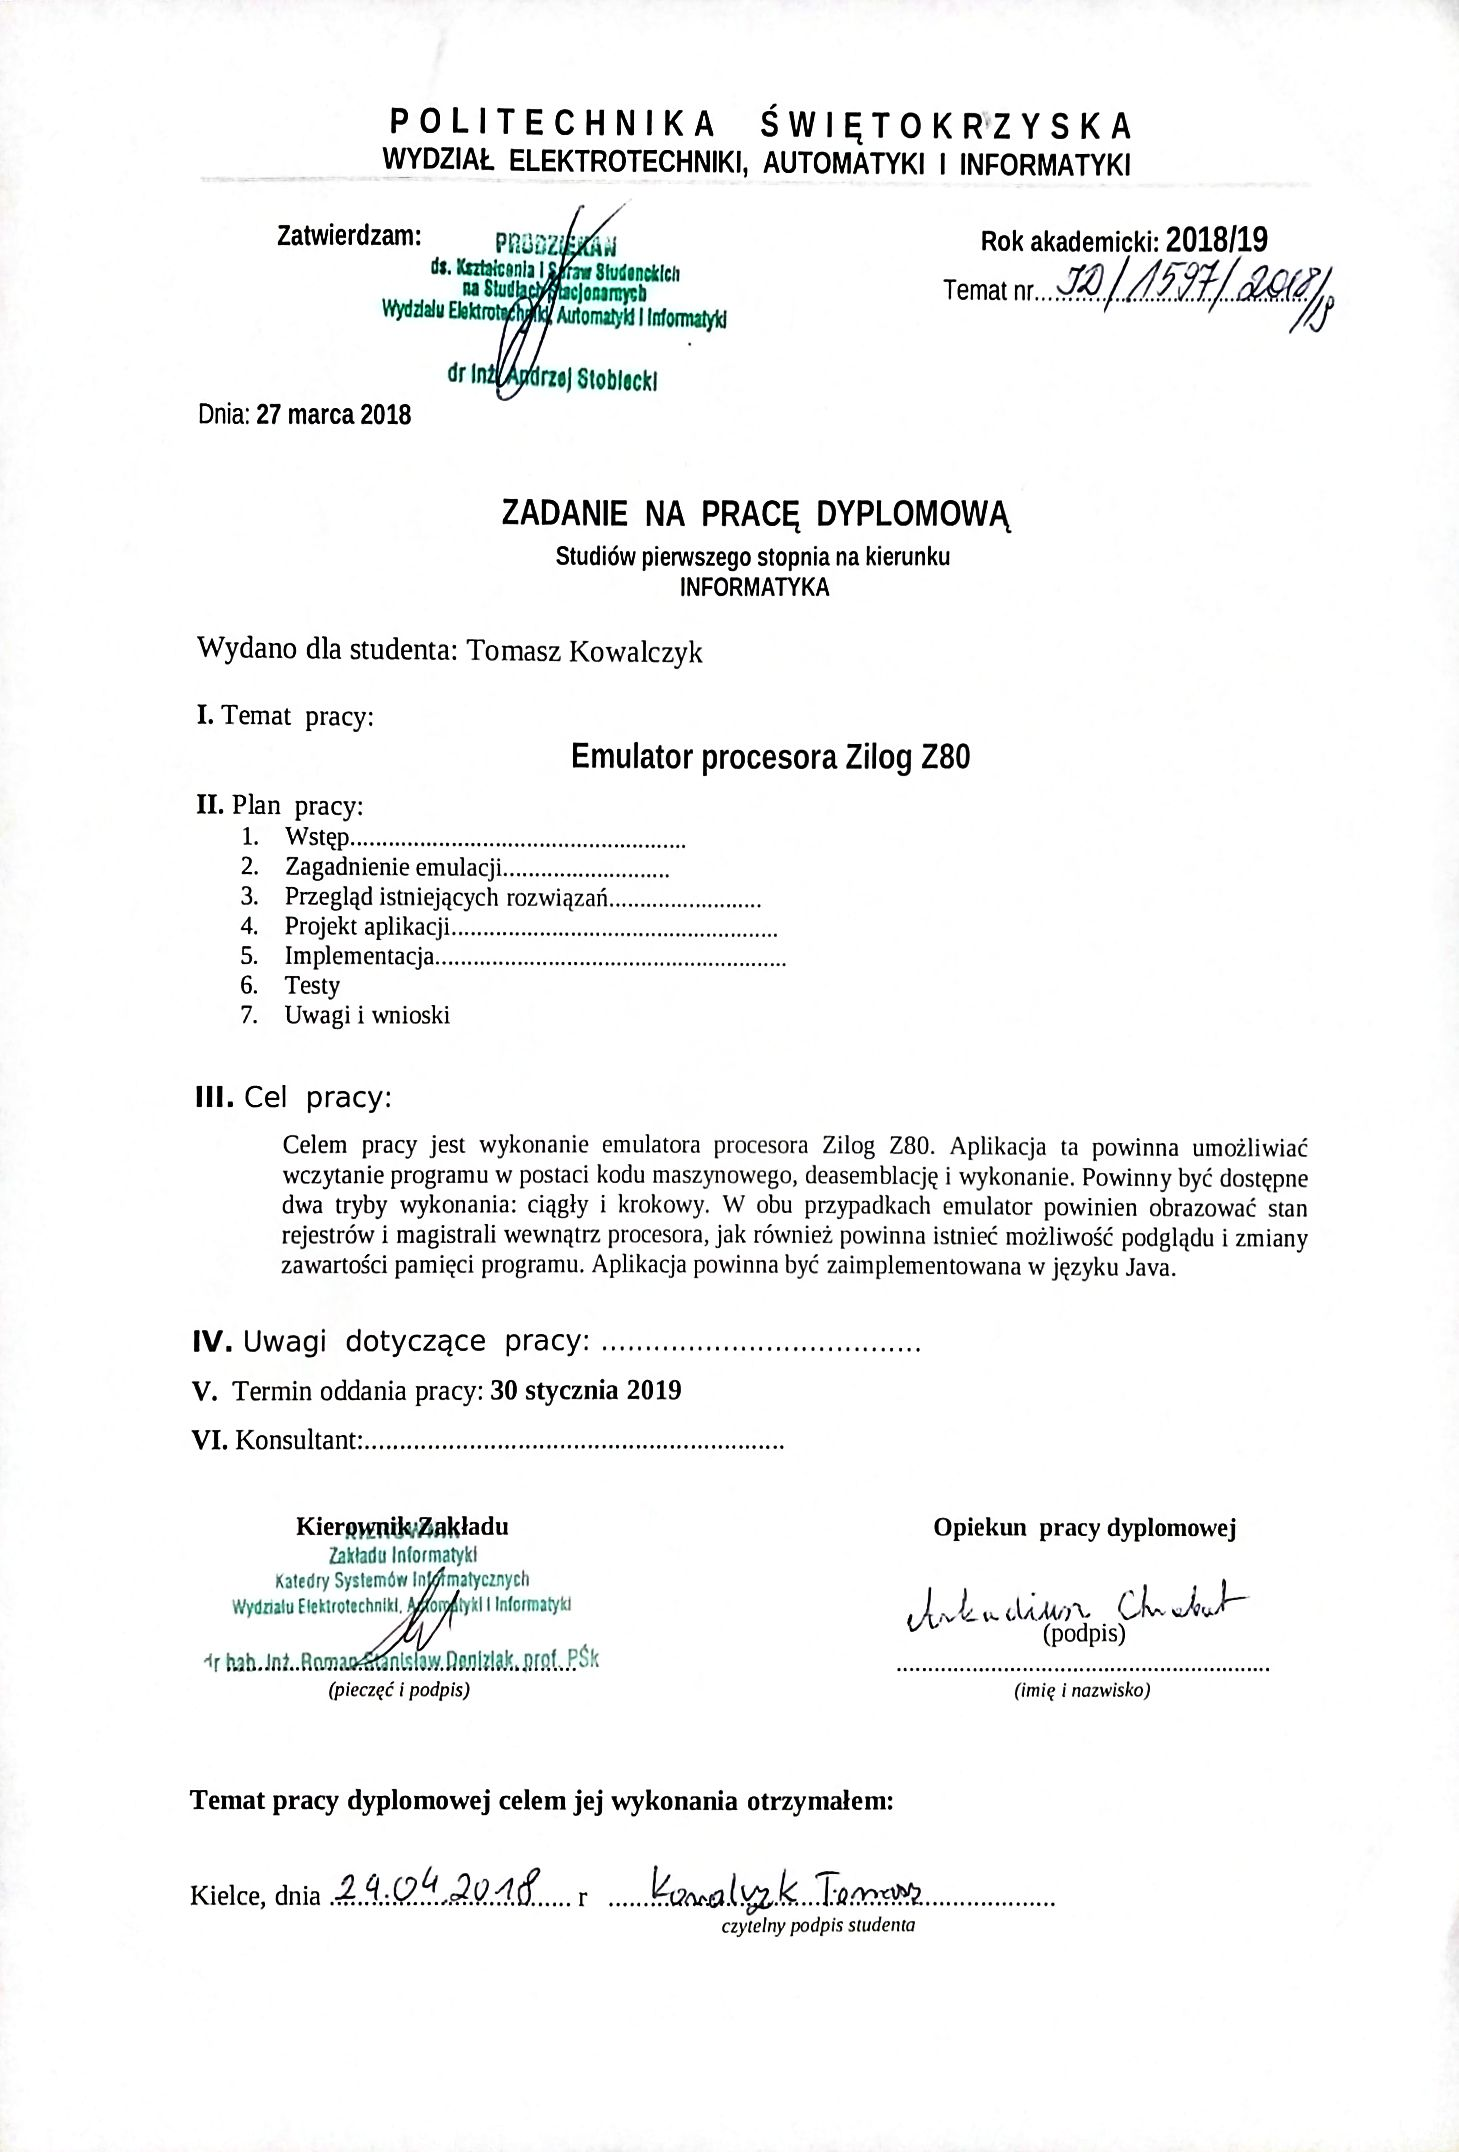
\includegraphics[width=1.0\paperwidth]{skany/zadanie.jpg}
	\end{figure}
	
	\leavevmode\thispagestyle{empty}\newpage
	
	\begin{figure}[H]
		\vspace{-2.5cm}
		\hspace{-3.5cm}
		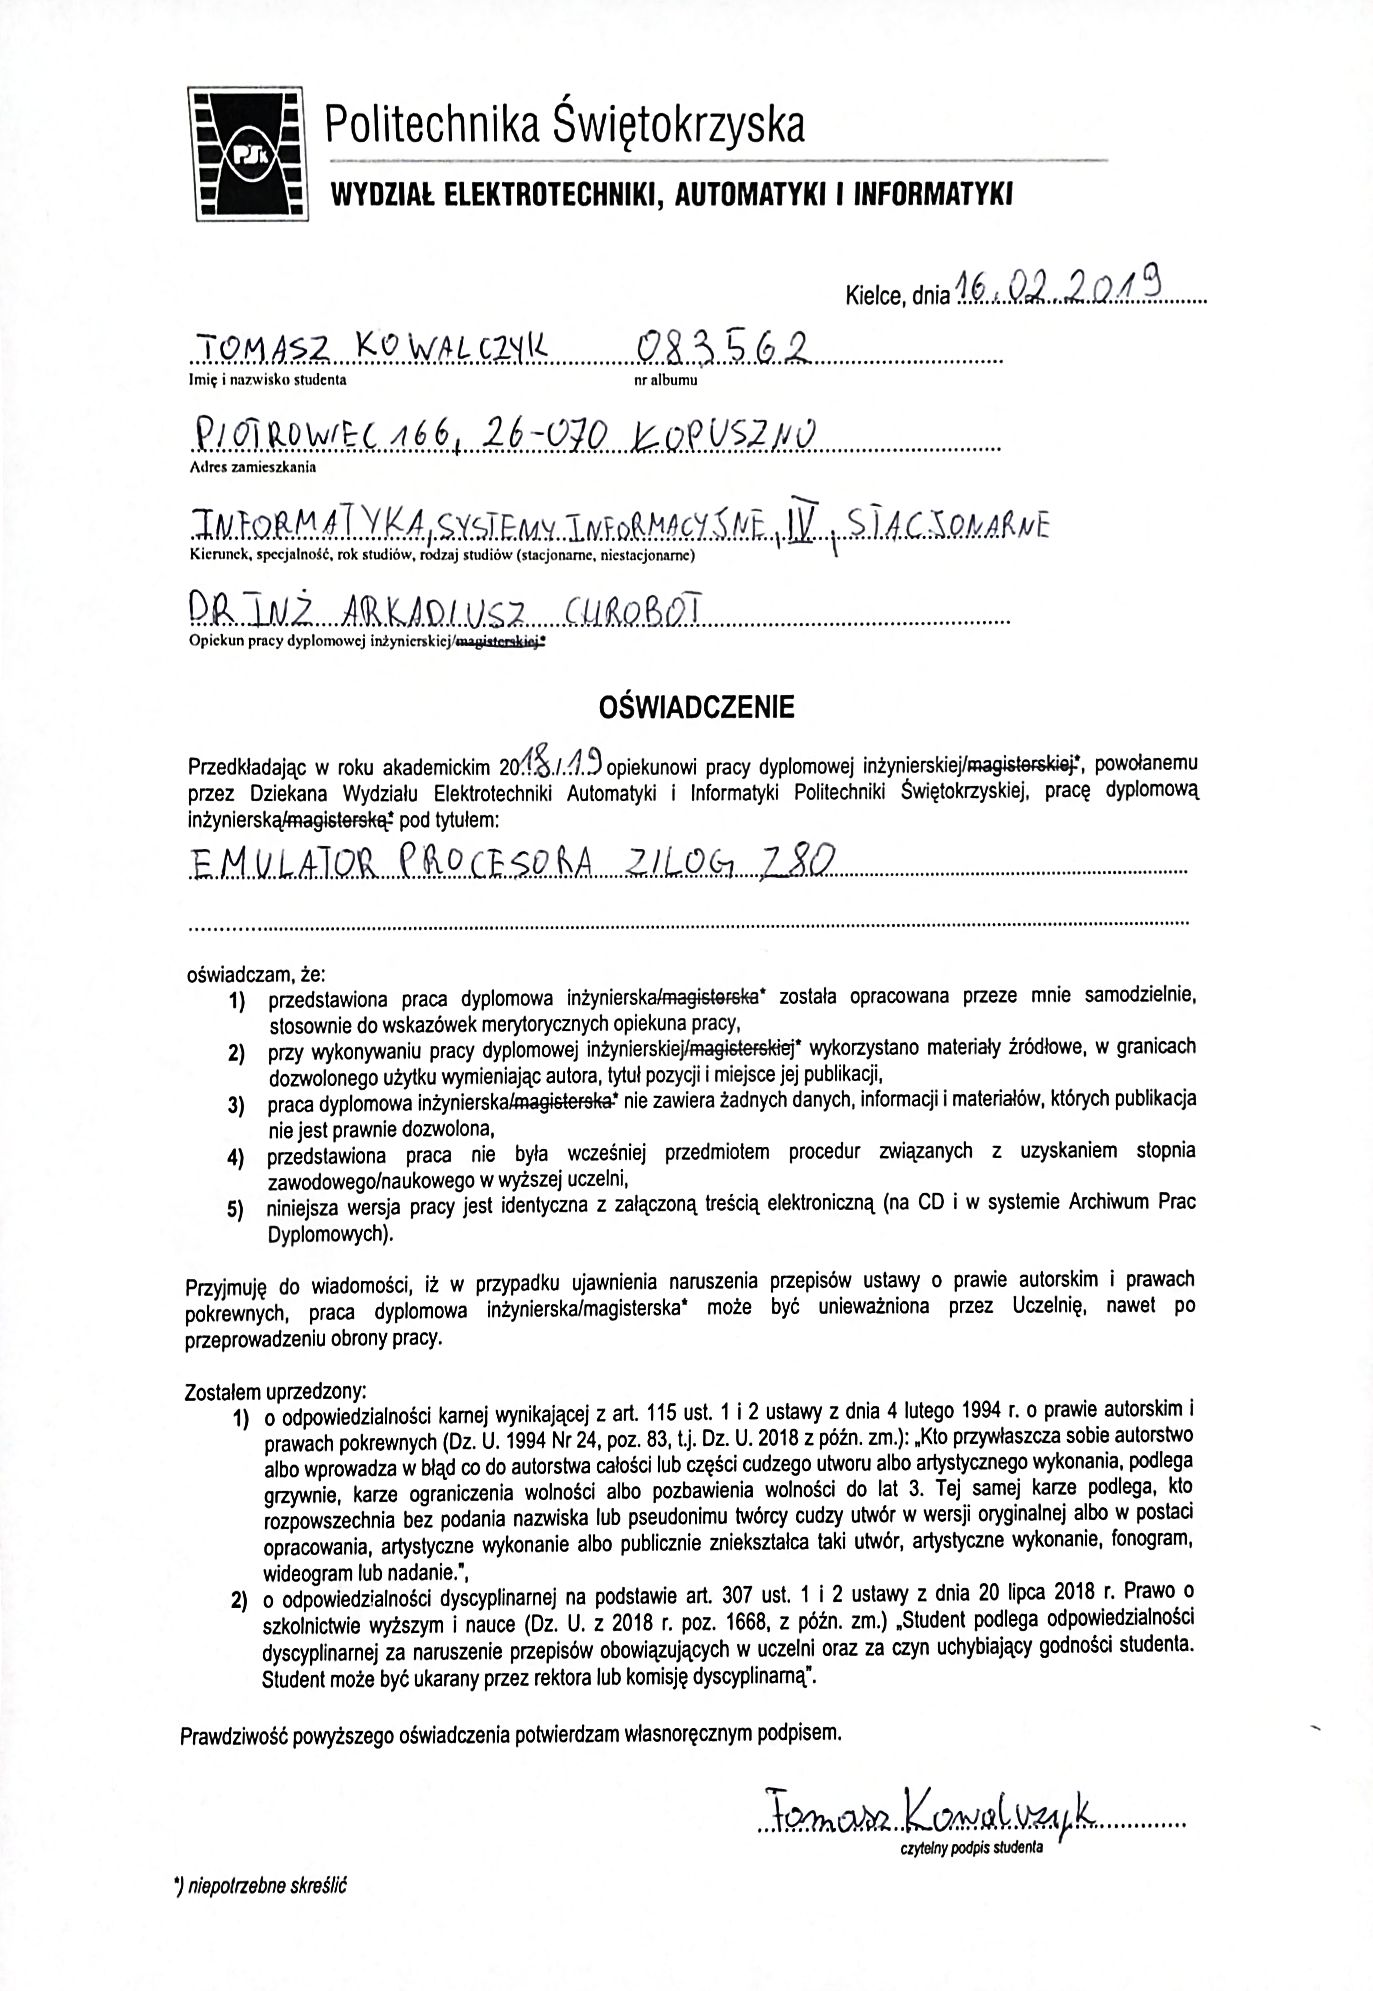
\includegraphics[width=1.0\paperwidth]{skany/osw.jpg}
	\end{figure}

	\leavevmode\thispagestyle{empty}\newpage
	
	\thispagestyle{empty}
\makeatletter
\begin{center}
	\large \textbf{\@title}
\end{center} 
\makeatother

\subsection*{Streszczenie}
Praca ma na celu ... \newline
Słowa kluczowe:
\begin{table}[!h]
\label{kluczowe}
\begin{tabular}{l l}

$\bullet$ Monitorowanie zasobów komputera       &       $\bullet$ Klaster \\
$\bullet$ Java 11                               &       $\bullet$ Spring boot 2 \\
$\bullet$ Angular 7                             &       $\bullet$ Linux \\

\end{tabular}
\end{table}

%\selectlanguage{english}
\makeatletter
\begin{center}
	\large \textbf{Internet application for monitoring cluster nodes}
\end{center} 
\makeatother

\subsection*{Summary}
The aim of the work is to develop an Internet application for monitoring.
Business layer of the application 
 made using Java 11 and the Spring Boot 2 framework  the MVC pattern, while the view layer was implemented Angular 7.
The application is divided into four modules: server - which authorizes users and aggregates data;
library that contains common classes used by server and agent;
an agent - which reports the status of the computer on which it is running to the server in a fixed time interval
and client that allows the user to view data on the server using a simple and clear interface based on dynamic websites.
\newline
Keywords:

\begin{table}[!h]
\label{keyword}
\begin{tabular}{l l}

$\bullet$ Monitoring computer resources         &       $\bullet$ Cluster \\
$\bullet$ Java 11                               &       $\bullet$ Spring boot 2 \\
$\bullet$ Angular 7                             &       $\bullet$ Linux \\

\end{tabular}
\end{table}
	
	\leavevmode\thispagestyle{empty}\newpage
	\leavevmode\thispagestyle{empty}\newpage
	
	%strona ze spisem treści
	\pagebreak
	\pagestyle{plain}
	\setcounter{page}{9} %start numeracji od strony 9
	\tableofcontents	 %generuj spis treści na podstawie \chapter i \section
	
	\leavevmode\newpage %pusta lub kontynuacja spisu treści
	
	\chapter*{Wstęp}
\addcontentsline{toc}{chapter}{Wstęp}
    
    % Celem pracy było zaimplementowanie emulatora procesora Ziloga Z80, dzięki któremu użytkownik mógłby w łatwiejszy sposób poznać jego architekturę.
    
    Celem pracy było zaimplementowanie emulatora procesora Zilog Z80. Emulator to program komputerowy, który duplikuje zachowania systemu komputerowego, za pomocą innego system komputerowego. \cite{studyofthetechniquesforemulationprogramming}
    W tym przypadku platformą docelową jest maszyna wirtualna Javy.
   %  W tym przypadku naśladowanym jest procesor Zilog Z80, a platformą docelową maszyna wirtualna javy.
    
	Procesor Zilog Z80 był bardzo popularny na rynku mikroprocesorów\cite{karczmarczuk}. 
	Stał się dostępny na rynku w~roku 1976 i~szybko zaczął być powszechnie stosowany w 8-bitowych systemach.
	
	Jedną z~przyczyn jego sukcesu, jest łatwy sposób sprzęgania go z innymi urządzeniami, szczególnie z kontrolerami pamięci. Inną jego zaletą jest lista rozkazów zgodna z~popularnym w tamtym czasie procesorem Intel 8080, co umożliwia uruchamianie programów napisanych pierwotnie dla tego procesora \cite{karczmarczuk}.
	
	Urządzenie to, mimo zalet, ma również poważne wady. Jego wewnętrzna budowa jest złożona jak na procesor ośmiobitowy. Piny magistrali danych nie są ułożone w logiczny sposób. Ich kolejność, jak ukazuje rysunek \ref{img:z80wyprowadzenia} (piny $D_{1} - D_{7} $) jest w losowej kolejności.
    
	\begin{figure}[h]
		\centering
		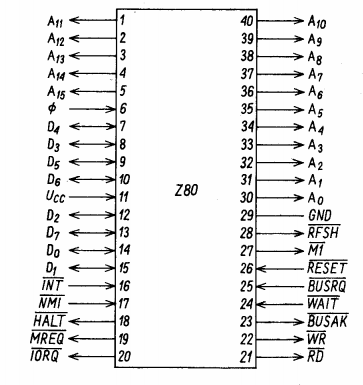
\includegraphics[width=0.5\textwidth]{z80wyprowadzenia}
		\caption{Wyprowadzenia mikroprocesora Z80 \cite{karczmarczuk}}
		\label{img:z80wyprowadzenia}
	\end{figure}
			
	
	\newpage
	Lista rozkazów procesora składa się z 158 pozycji, w tym 78 z nich jest zgodnych z~Intel 8080\cite{manual}. Poznanie działania każdego z nich jest trudne i czasochłonne dla większości osób. Omawiany projekt emulatora ma na celu, oprócz samego wykonywania kodu programu, prezentować zmiany jakie zachodzą wewnątrz procesora. Użytkownik może prześledzić proces wykonywania dowolnej instrukcji i sprawdzić jak wpływa ona na~pamięć, rejestry, czy flagi procesora. Wszystkie te wewnętrzne parametry można modyfikować podczas procesu emulacji, za pomocą graficznego interfejsu użytkownika, zaprezentowanego w~rysunku \ref{img:z80Gui}.
	
	W rozdziale pierwszym opisano proces emulacji oraz trzy sposoby jej wykonania, z~naciskiem na metodę wybraną w projekcie.
	
	Rozdział drugi zawiera przegląd wybranych emulatorów Zilog-a Z80. Skupiono się głównie na aplikacjach zawierających graficzny interfejs użytkownika tak jak opisywany projekt. 
    
    %@todo dokładniej opisać co przedstawia projekt aplikacji
    Rozdział trzeci przedstawia projekt aplikacji, wymagania funkcjonalne i niefunkcjonalne, oraz podział na moduły.
	
	Rozdział czwarty opisuje implementacje poszczególnych modułów projektu. Wyjaśniono sposób wykonywania emulacji, realizacje operacji bitowych, oraz sposób integracji poszczególnych części aplikacji.
	
	
	W rozdziale szóstym zawarto informacje na temat testów jednostkowych i manualnych aplikacji użytych w celu sprawdzenia poprawności wykonywania emulacji.
	
	W rozdziale siódmym podsumowano projekt oraz opisano ewentualne możliwości rozwoju.
	\chapter{Zagadnienie emulacji}

    W rozdziale tym wyjaśniono, czym jest proces emulacji, na czym polega, oraz w jaki sposób może zostać on zaimplementowany. Zwrócono także uwagę na różnicę między pojęciami \emph{symulacja} oraz \emph{emulacja}, które są często błędnie używane zamiennie.

	Emulator w~dziedzinie informatyki, oznacza program który jest przystosowany do uruchomienia w~określonym systemie komputerowym i pozwala na wykonywanie programów przeznaczonych dla innego tego typu urządzenia\cite{howDoIWriteAnEmulator}. 
	
	Inną ciekawą definicję emulatora podał Victor Moya del Barrio ,,Emulator to program komputerowy, którego zadaniem jest symulacja zachowania wszystkich komponentów danego urządzenia, używając oprogramowania uruchamianego na innym urządzeniu" 
	\cite{studyofthetechniquesforemulationprogramming}.
		
	Emulacje CPU można przeprowadzić na trzy sposoby:\cite{fms_komkon_org_howto}	
	\begin{itemize}  
		\item przez interpretowanie,
		\item przez statyczną rekompilację,
		\item przez dynamiczną rekompilację.
	\end{itemize} 
	Każda z tych metod wymaga oddzielnego przedstawienia.
	
	\section{Emulacja przez interpretowanie}
	Interpreter to najprostszy rodzaj emulatora. Odczytuje on w pętli kod programu z~symulowanej pamięci. Odczytany bajt (lub bajty, gdyż rozkaz procesora może być wielobajtowy) zawiera informacje o rodzaju operacji jaką CPU 
	powinien wykonać. Interpreter ma za zadanie odkodować informacje o operacji, a następnie ją wykonać. Między wykonaniem kolejnych rozkazów powinien on zmienić wirtualne parametry (np. zwiększyć o~jeden wartość licznika rozkazów), sprawdzić czy nie zostało zgłoszone przerwanie, obsłużyć urządzenia wejścia/wyjścia, liczniki, kartę graficzną, lub wykonać inne operacje zależne od emulowanego urządzenia. Schemat struktury interpretera został przedstawiony na listingu \ref{listing:interpreter}.
	
	\begin{listing}[h]
		\inputminted{java}{listings/interpreter.c}
		\caption{Schemat struktury interpretera procesora}
		\label{listing:interpreter}
	\end{listing}
		
	Emulacja przez interpretowanie jest najwolniejszą formą emulacji, ale także najłatwiejszą w debugowaniu. Pozwala ona na prześledzenie wykonania operacji i podgląd wewnętrznych stanów urządzenia. Z tego powodu jest najczęściej wybierana przez programistów do tworzenia debuggerów procesorów oraz mikrokontrolerów.
	
	\section{Statyczna rekompilacja}
	Statyczna rekompilacja (ang. \emph{static binary translaion}) to proces konwertowania kodu maszynowego na inny kod maszynowy przeznaczony dla docelowej platformy sprzętowej. Plik wykonywalny tłumaczony jest w~całości i~tylko raz. Wadą tego rozwiązania są problemy z~tłumaczeniem rozkazów skoków pośrednich czyli takich gdzie adres skoku przechowywany jest w rejestrze lub pamięci i może on być uzyskany tylko podczas wykonywania programu. W takim przypadku niemożliwym jest przetłumaczenie wszystkich instrukcji pliku wykonywalnego\cite{uqbt}. 
	
	
	\section{Dynamiczna rekompilacja}
	Dynamiczna rekompilacja (ang. \emph{Dynamic binary translator}), w odróżnieniu od translacji statycznej, tłumaczy kod blokami podczas jego wykonywania. Dokonywana jest ona ,,na żądanie" w~związku z~tym jest wolniejsza od rekompilacji statycznej, ale rozwiązuje problem związany z tłumaczeniem rozkazów skoków pośrednich.
	
	Raz przetłumaczony fragment kodu jest przechowywany w pamięci, na wypadek potrzeby jego ponownego użycia, co pozwala zwiększyć efektywność tej metody emulacji\cite{uqbt}.
	
	Dynamicznej rekompilacji używa w dużym stopniu maszyna wirtualna języka Java. Wczesne wersje JVM (ang. \emph{Java Virtual Machin}) używały interpreterów, co okazało się mało wydajne. Dobrym sposobem na poprawę efektywności maszyny wirtualnej Java jest dynamiczne tłumaczenie kodu bajtowego\cite{dynamicRecompilationInJava}. 
	
	\section{Różnica między symulacją a emulacją} 
	Różnicę między emulacją a~symulacją obrazuje tabela \ref{table:emulationAndSimulation}.
	
	\begin{table}
		\centering
		\begin{tabular}{ m{7cm} | m{7cm} }
			Symulator &  Emulator  \\ 
			\hline
			System zdolny do naśladowania innego systemu w pewnym stopniu.  & System który naśladuje dokładne zachowanie innego systemu. \\   
			\hline
			Może nie przestrzegać wszystkich reguł symulowanego systemu. & Ściśle przestrzega parametrów i reguł emulowanego systemu. \\ 
			\hline
			Modeluje aplikacje i zdarzenia. & Kopiuje zachowanie systemów. \\ 
		\end{tabular}
		\caption{Różnice między symulacją a emulacją \cite{emulationOrSimulation}}
		\label{table:emulationAndSimulation}
	\end{table}
	
	W~informatyce, symulator to program komputerowy, który modeluje zachowania i~funkcje innego realnego systemu lub zjawiska (np. prowadzenie pojazdu). Nie jest wymagane, aby odwzorowywał wszystkie jego zachowania i~funkcje. Symulator nie wykonuje realnych zadań symulowanego urządzenia i ~nie zastępuje go\cite{emulationOrSimulation}.
	
	Natomiast emulator ma za zadanie ,,udawać" dane urządzenie/zjawisko w takim stopniu~i na takim poziomie, aby był w stanie zastąpić emulowane urządzenie i funkcjonować tak jak ono\cite{emulationOrSimulation2}.
	
	W~rozdziale zdefiniowano, czym jest emulacja w dziedzinie informatyki. Przybliżono jej realizacje przez interpretacje oraz statyczną i dynamiczną rekompilacje. Na koniec zwrócono uwagę, że wbrew powszechnej opinii emulacja i symulacja nie są synonimami, oraz wytłumaczono różnicę między nimi.

	% linki z których czerpałem wiedze:
	% https://www.guru99.com/real-device-vs-emulator-testing-ultimate-showdown.html
	% http://fms.komkon.org/EMUL8/HOWTO.html https://stackoverflow.com/questions/1584617/simulator-or-emulator-what-is-the-difference
	% https://www.quora.com/What-are-the-differences-between-simulation-and-emulation
	% TO NAJLEPSZE: https://softwareengineering.stackexchange.com/questions/134746/whats-the-difference-between-simulation-and-emulation
		
	% W książe "Study of the techniques for emulation programming" Victor Moya del Barrio podaje taką to definicje emulatora "An emulator tries to duplicate the behaviour of a full computer using software programs in a different computer."\cite{studyofthetechniquesforemulationprogramming}. https://www.overleaf.com/project/5c58bbe8b206d66446cbcd63
	\chapter{Przegląd istniejących rozwiązań}
	Procesor Zilog Z80 jest często emulowany, ze względu na jego dużą popularność. Emulatory tworzone są zarówno przez duże firmy, jak i hobbystów. Na platformie \emph{Github}  która jest przeznaczona dla projektów programistycznych, można znaleźć około dwustu repozytoriów z projektami emulującymi Z80, lub urządzenia używające tego procesora. %\cite{githubZ80Emulators}

	W~tym rozdziale zaprezentowane są najciekawsze emulatory, które posiadają graficzny interfejs użytkownika i pozwalają na wgląd w wewnętrzne stany procesora (czyli najbardziej przypominające zakresem swoich funkcji aplikację będącą przedmiotem tej pracy). Przedstawione są zarówno komercyjne rozwiązania, jak i te pisane przez amatorów.
	
	\section{Z80 SIMULATOR IDE}
	Jest to dostępny pod adresem http://www.oshonsoft.com/z80.html płatny emulator posiadający najbardziej rozbudowany interfejs z wszystkich opisanych programów. 
	Pozwala on na prezentowanie wewnętrznych stanów procesora, manipulację przerwaniami i portami wejścia/wyjścia. Zawiera edytor pamięci działający również podczas emulacji. 
	Posiada on również funkcje i~elementy typowe dla debuggerów, jak możliwość wstrzymania działania programu w określonym miejscu, tryb pracy krokowej, interaktywny edytor i~kompilator kodu asemblera\cite{oshonsoftEmulator}. Widok interfejsu użytkownika tego programu jest zaprezentowany na rysunku \ref{img:oshonsoftEmulator}.
	
	\begin{figure}[h]
		\centering
		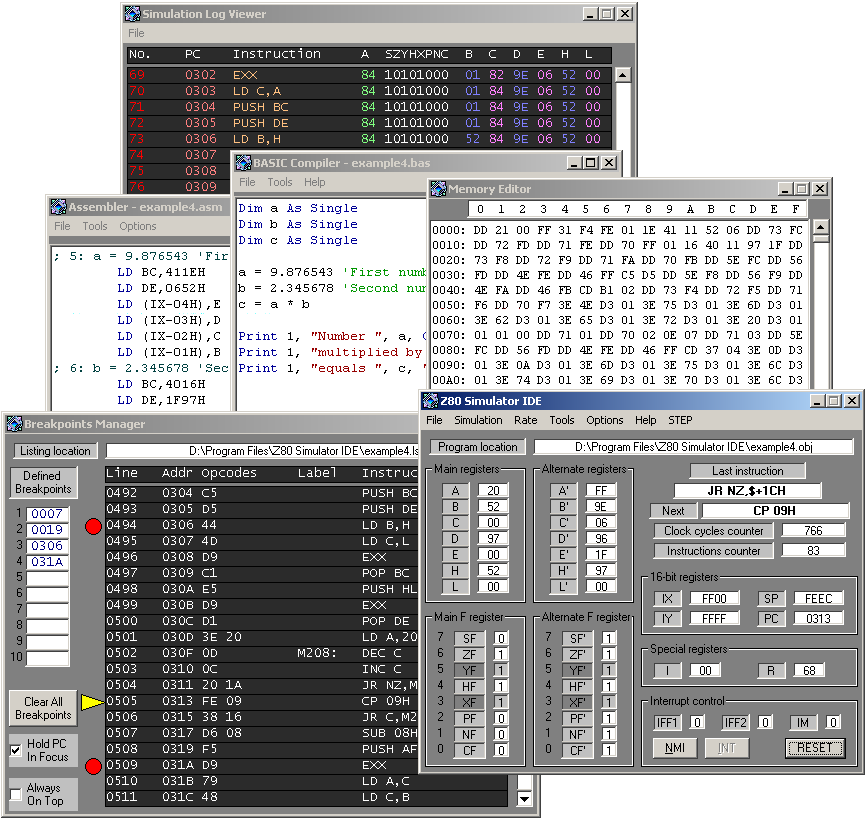
\includegraphics[width=0.7\textwidth]{oshonsoftEmulator}
		\caption{Z80 SIMULATOR IDE}
		\label{img:oshonsoftEmulator}
	\end{figure}
	
	Jedną z wad emulatora Z80 SIMULATOR IDE jest interfejs, który nie jest intuicyjny. Przykładowo, autorzy programu nie umieścili w~nim informacji, o tym w jakim formacie powinny być wprowadzane wartości liczbowe. Brak w programie systemu pomocy i opisów, co może znacznie utrudniać pracę początkującym użytkownikom. Dodatkowo jest to narzędzie płatne, przeznaczone dla specjalistów i~uruchamiane tylko w~systemie MS Windows.
	
	
	\section{ZEMU - Z80 Emulator Joe Moore}
	ZEMU to emulator zaprojektowany głównie po to, aby umożliwiać uruchamianie systemu operacyjnego CPM, który był oferowany przez firmę \emph{Digital Research Inc.} w~latach 1970{\dywiz}1980\cite{cpm}. Program skierowany jest do hobbystów. Oprócz standardowych możliwości takich jak podgląd, edycja zawartości pamięci, rejestrów i flag, może on również emulować stację dyskietek, port COM, szeregowy, monitor CRT i~drukarkę.    
	
	Rysunek \ref{img:zemu} przedstawia interfejs aplikacji. Tak, jak w przypadku Z80 SIMULATOR IDE nie jest on intuicyjny, brak mu systemu pomocy, jego elementy nie są opisane w wystarczającym stopniu. Osoby nie mające doświadczenia z urządzeniami wejścia/wyjścia w Zilogu Z80 będą miały problem z obsługą nawet podstawowych funkcji.
	
	Inną wadą aplikacji jest brak możliwości jej uruchomienia w~innym systemie operacyjnym niż \emph{Windows}. 
	
	\begin{figure}[h]		
		\centering
		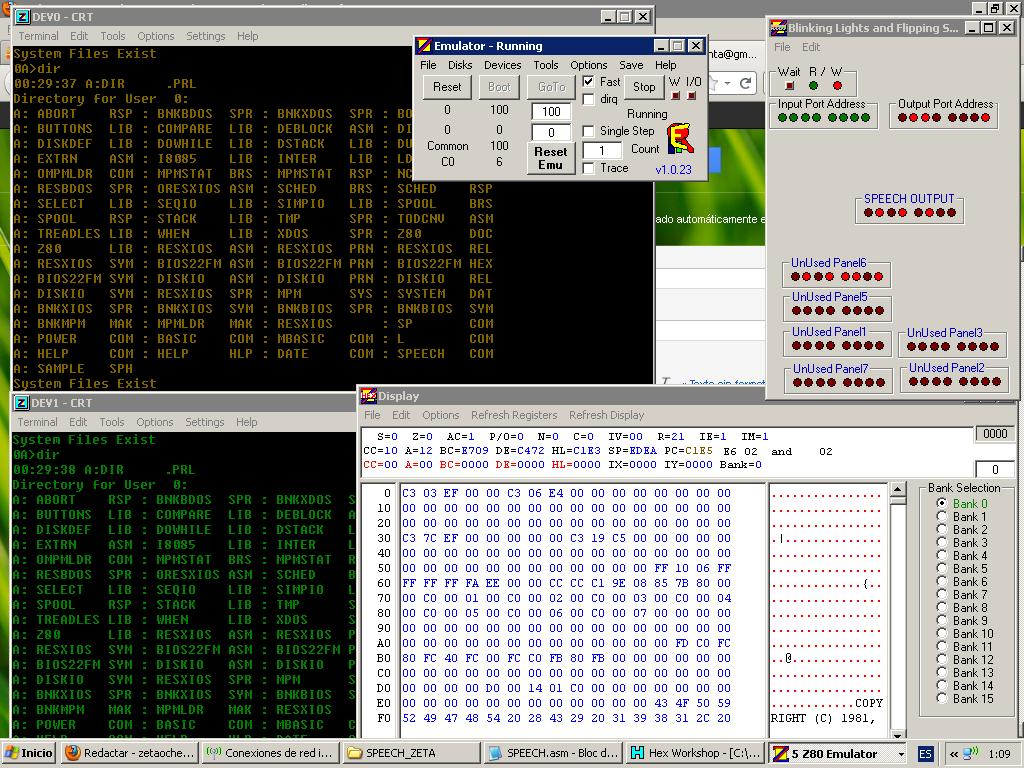
\includegraphics[width=0.8\textwidth]{zemu}
		\caption{ZEMU}
		\label{img:zemu}
	\end{figure}
	
	 \section{ZIM - The Z80 Machine Simulator}
	ZIM został napisany z~użyciem technologii \emph{Java Web-Start}. Pozwala ona na uruchomienie aplikacji bezpośrednio na stronie internetowej, ale również pozwala na dostęp do lokalnych zasobów komputera, np. plików. 
	Aplikacja według autora przeznaczona jest głównie dla studentów uczących się języka asemblera dla procesora Z80\cite{zimManual}.
	
	Program pozwala na podgląd wszystkich wewnętrznych parametrów CPU, emuluje proste urządzenia wejścia/wyjścia, umożliwia edycję zawartości pamięci, debugowanie programu dla procesora Z80 i~symulację przerwań. Zaletą emulatora jest możliwość jego uruchamiania na wielu platformach sprzętowych, dzięki zastosowaniu języka Java.
	
	W~aplikacji brakuje natomiast edytora asemblera i~systemu pomocy. Interfejs użytkownika ma wiele defektów i nie jest intuicyjny. Na rysunku \ref{img:zim} przedstawiono zrzut ekranu działającej aplikacji.
	
	\begin{figure}[h]		
		\centering
		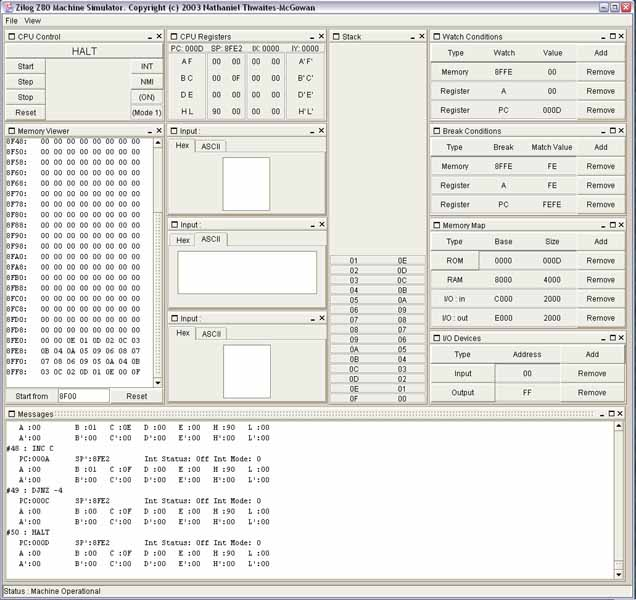
\includegraphics[width=0.8\textwidth]{zim}
		\caption{ZIM - The Z80 Machine Simulator}
		\label{img:zim}
	\end{figure}
	
	%Żadne istniejące rozwiązanie nie pozwala na podejrzenie wewnętrznych magistrali procesora
	
	\section{Podsumowanie istniejących rozwiązań}
	Problemem prawie wszystkich emulatorów i symulatorów jest ich interfejs użytkownika. Ta uwaga dotyczy nie tylko emulatorów konkretnie omawianego procesora, ale ogółu tego typu aplikacji. Są one przeznaczone dla osób znających architekturę komputerową, oraz budowę i działanie konkretnego emulowanego urządzenia. Z~tego powodu programiści nie przywiązują odpowiedniej wagi do intuicyjności i systemów pomocy dla interfejsów użytkownika. Osoby nieposiadające wymaganej wiedzy albo znające jedynie podstawy zagadnienia nie są w stanie sprawnie obsługiwać programu. 
	
	Emulatory nie są przeznaczone do uruchamiania na wielu platformach sprzętowych. Dotyczy to szczególnie aplikacji emulujących przez rekompilację. Do jej wykonania wymagana jest znajomość architektur wyjściowej i docelowej maszyny. Rozwiązaniem tego problemu mogą być interpretery napisane w języku Java, takie jak ,,ZIM - The Z80 Machine Simulator". Rozwiązanie to wykorzystuje dużo zasobów procesora. Kod przeznaczony dla emulowanej maszyny jest najpierw interpretowany przez interpreter napisany w języku Java, a następnie ponownie emulowany już za pomocą dynamicznej rekompilacji w maszynie wirtualnej. Typowe rozwiązania napisane w języku kompilowanym dla konkretnego procesora działają szybciej, kosztem możliwości uruchamiania na wielu platformach sprzętowych. Wydajność maszyny wirtualnej języka Java nie jest przeszkodą do stworzenia w~tym języku emulatora procesora Zilog Z80. Współczesne komputery są na tyle efektywne, że taki emulator może pracować z~wydajnością zbliżoną do wydajności oryginalnej maszyny.
	
	Kolejną kwestią o której warto wspomnieć jest czytelność kodu emulatorów. Kod istniejących rozwiązań nie należy do łatwych do zrozumienia. Najczęściej cały program w~postaci źródłowej emulatora zawiera się w jednym pliku o~wielkości kilkuset wierszy. Osoba chcąca przestudiować proces emulacji ma zatem utrudnione zadanie.
	
	Podsumowując, aktualnie brakuje wieloplatformowego emulatora lub symulatora Ziloga Z80, z czytelnym, poprawnie działającym interfejsem użytkownika, czytelnym, dobrze opisanym kodem źródłowym i~użytecznym systemem pomocy.
	
	\chapter{Projekt aplikacji}
	Podczas projektowania aplikacji, ustalono jej wymaganie funkcjonalne oraz niefunkcjonalne. Opracowano strukturę projektu, która zakłada podział programu na trzy mniejsze części. Zamieszczono diagramy UML przedstawiające publiczne interfejsy programistyczne tych modułów.
	
	\section{Wymagania funkcjonalne}
	Założono, że aplikacja będzie posiadać graficzny interfejs użytkownika umożliwiający podgląd i modyfikacje stanów wewnętrznych procesora, takich jak rejestry, pamięć i~flagi. Możliwe będzie wykonanie dwóch trybów emulacji, ciągły oraz krokowy. 
	W widocznym miejscu zostaną umiejscowione informacje o liczbie wykonanych cykli maszynowych i zegara.
	Aplikacja pozwoli na zgłaszanie przerwań maskowalnych i niemaskowalnych oraz wprowadzenia wartości szyny danych, jaką ustaliłoby urządzenie wywołujące przerwanie podczas zgłoszenia. 
	Użytkownikowi zostanie udostępniona możliwość wprowadzenia kodu asemblera do aplikacji, skompilowanie go i wczytanie do pamięci. Podczas emulacji zostanie wyświetlona nazwa poprzedniej i następnej wykonanej instrukcji procesora.

	\section{Wymagania niefunkcjonalne}
	Podstawowym założeniem, jest możliwość uruchomienia aplikacji na jak największej liczbie platform. Jako minimum zdecydowano się na systemy operacyjne \emph{MS Windows}, \emph{Ubuntu} i \emph{Mac OS}. Instrukcje procesora powinny być wykonywane bezbłędnie, zgodnie z dokumentacją techniczną procesora. Projekt powinien mieć interfejs programistyczny umożliwiający podłączenia go z innymi aplikacjami, np. emulatorami urządzeń, które do swojej pracy wykorzystują Ziloga Z80.
	
	\section{Struktura aplikacji}
	Aplikację podzielono na trzy moduły: \emph{Xbit}, \emph{Z80emu{\dywiz}core} oraz \emph{Z80emu{\dywiz}gui}, z~których każdy jest osobnym modułem. Zależności między nimi pokazuje diagram \ref{img:strutkuraAplikacji}. Moduł \emph{XBit} do swojego działania nie wymaga innych modułów. \emph{Z80emu{\dywiz}core} potrzebuje modułu \emph{XBit} do poprawnego działania i jest on jego częścią, natomiast \emph{X80emu{\dywiz}gui} zawiera w sobie \emph{Z80emu{\dywiz}core}, a co za tym idzie także \emph{Xbit}.
    
    \begin{figure}[h]
		\centering
		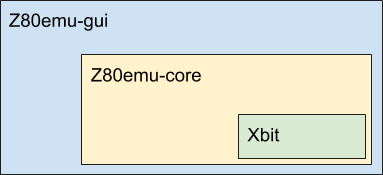
\includegraphics[width=0.6\textwidth]{strukturaAlikacji.png}
		\caption{Zależności pomiędzy modułami aplikacji}
		\label{img:strutkuraAplikacji}
	\end{figure}
    
	\section{Biblioteka XBit}
	Java jest językiem programowania wysokiego poziomu, kompilowanym do kodu bajtowego. Z tego powodu nie jest on zazwyczaj stosowany w emulacji, gdyż kod emulatora musi być uruchamiany w maszynie wirtualnej, co nie jest wydajnym rozwiązaniem.

	Innym poważnym problemem języka Java jest brak typów prostych pozwalających przechowywać wyłącznie liczby dodatnie. Problem rozwiązuje biblioteka XBit. Zawiera ona klasy, które umożliwiają przechowywanie wartości jedno i dwu bajtowych. Mogą one zostać zinterpretowane jako liczby zapisane w kodzie dopełnień do dwóch (liczby dodatnie i ujemne), lub naturalnym kodzie binarnym (tylko liczby dodatnie). \newline
	Przykładowo, liczba binarna 1110 odczytana w naturalnym kodzie binarnym (NKB), to 15 (w zapisie decymalnym), natomiast w kodzie dopełnień do dwóch (U2) to -2. XBit pozwala na obydwie interpretacje za pomocą odpowiednich metod, zwracając wynik jako typ prymitywny \emph{int}. 
	
	Nie jest to idealne rozwiązanie. Typ \emph{int} przechowuje cztero{\dywiz}bajtowe liczby z zakresu od -2 147 483 648 do 2 147 483 647, więc większość bajtów zostaje niewykorzystana. Nadmiarowość jest w tym przypadku wymagana, ponieważ zakres liczb w notacji NKB i~w~U2 jest inny.
	
	Przykładowo, w przypadku gdy za pomocą XBit stworzono reprezentację liczby ośmio bitowej: \newline1111 0000 (w kodzie jest to NKB=240, U2=-16) to wywołując metodę interpretującą ją jako liczba bez znaku (czyli w notacji NKB), zostanie zwrócona zmienna o typie prymitywnym \emph{int}, o wartości 240,  binarne \newline 00000000 00000000 00000000 11110000. \newline
	Natomiast jeśli wykonamy metodę interpretującą ją jako liczba ze znakiem (czyli w notacji U2) zostanie zwrócona wartość -16, binarnie \newline 11111111 11111111 11111111 11110000.\newline
    
    Bibliotekę zaprojektowano w taki sposób, aby była jak najbardziej uniwersalna, i można ją było wykorzystać do budowy emulatora Zilog-a Z80, ale także innych procesorów. 

	\subsection{Możliwości biblioteki XBit}
	Założono, że biblioteka \emph{XBit} będzie spełniała następujące wymagania:
	\begin{itemize}  
		\item reprezentacja liczb 8 i 16 bitowych,
		\item interpretacja liczb w naturalnym kodzie binarnym lub dopełnieniu do dwóch,
		\item operacje na pojedynczych bitach (możliwość zmiany, odczytu bitu na danej pozycji),
		\item opcja odczytania grupy bitów (odczytanie kilku bitów z~określeniem pozycji pierwszego i ostatniego bitu),
		\item interpretacja liczb 16 bitowych w formacie \emph{big endian} lub \emph{little endian},
		\item operacje arytmetyczne (dodawanie, odejmowanie),
		\item operacje bitowe na liczbach (negacja, alternatywa, koniunkcja, przesunięcia bitowe),
		\item uwzględnienie przy operacjach arytmetycznych przepełnienia oraz przeniesienia.
	\end{itemize} 
	
	\subsection{Założenia projektowe XBit}
	Przed przystąpieniem do implementacji rozwiązania, zaprojektowano publiczny interfejs biblioteki w języku UML, zaprezentowany na diagramie \ref{img:xbitUml}. Ustalono także założenia projektowe, które zaprezentowano poniżej. 
	
	\begin{figure}[h]
		\centering
		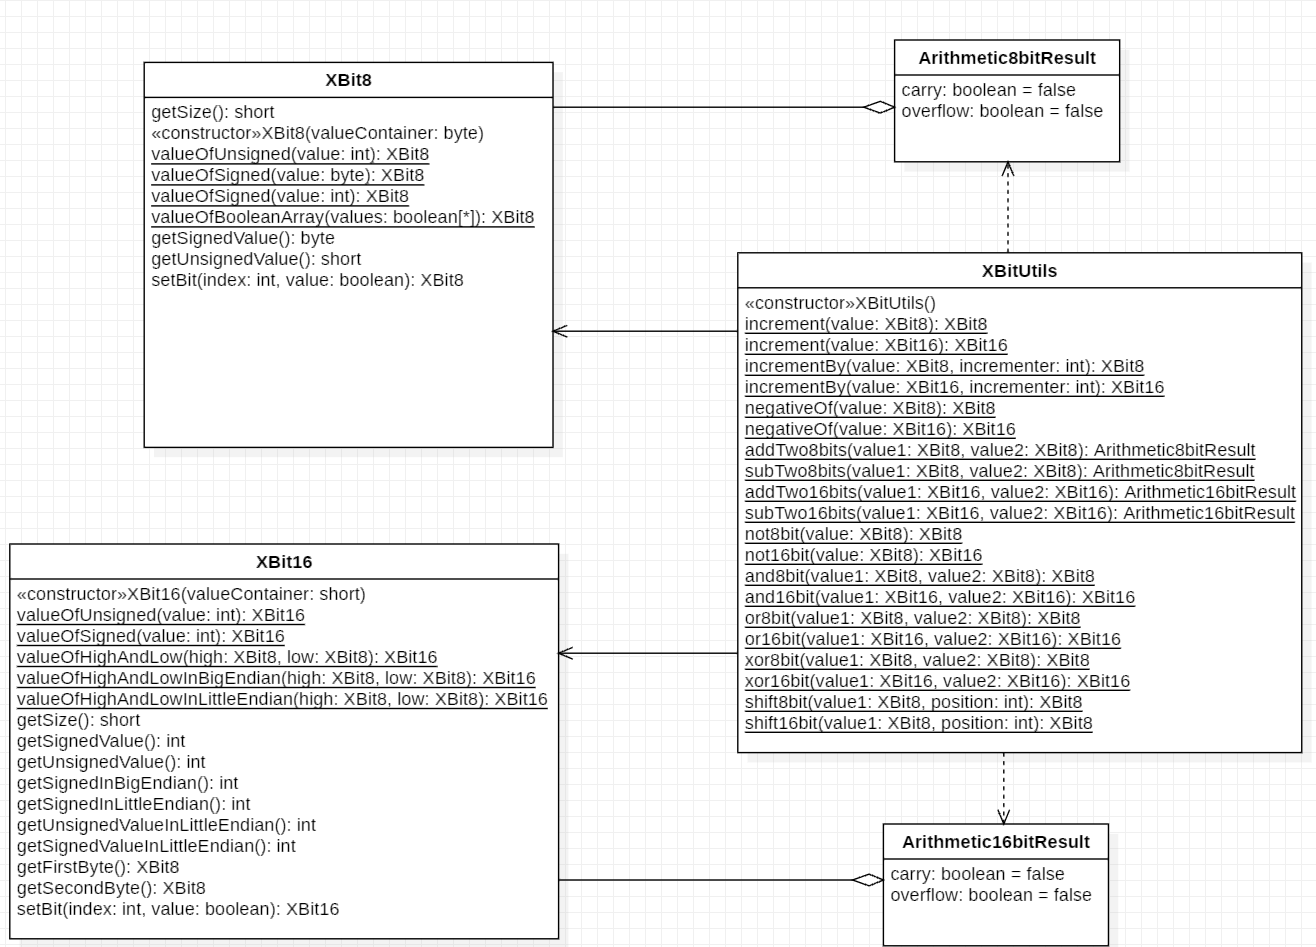
\includegraphics[width=1\textwidth]{xbitUml}
		\caption{Hierarchia klas biblioteki XBit}
		\label{img:xbitUml}
	\end{figure}
	
	\subsubsection{Klasy XBit8 i XBit16}
	Klasy \emph{XBit8} oraz \emph{XBit16} służą do reprezentowania liczb 8 i 16 bitowych. Postanowiono, że zmiana stanu wewnętrznego ich obiektów, czyli wartości w~nich przechowywanych będzie niemożliwa (są to obiekty niezmienne, z ang. \emph{immutable}), tak jak w~przypadku obiektowych reprezentacji typów prostych w języku Java (\emph{Short}, \emph{Long}, \emph{Integer} itp).  Konsekwencją tej decyzji jest to, że metody które powinny zmienić stan obiektu, klonują istniejący obiekt a następnie modyfikują odpowiednio stan jego kopii. Przykładem takiej metody jest \emph{setBit(index: int, value: boolean)} występująca w~obu klasach. Podprogram ten nie zmienia bitu obiektu na rzecz którego został wykonany, a jedynie zwraca kopie obiektu, ze zmodyfikowanym odpowiednim bitem. 
	
	Zalety zastosowania obiektów niezmiennych:
	\begin{itemize} 
		\item prosta implementacja oraz łatwe debugowanie kodu,
		\item \emph{Garbage Collector} jest przystosowany do pracy z tego typu obiektami,
		\item łatwość zapisywania obiektów do pliku lub pamięci podręcznej (z ang. \emph{cache}),
		\item bezpieczne używanie obiektów niezmiennych w programach wielowątkowych, co ułatwia emulacje procesorów wielopotokowych; jeden wątek w takim przypadku mógłby być odpowiedzialny za jeden stopień potoku, np osobny wątek odbierałby instrukcje z pamięci, inny by je dekodował, kolejny wykonywał i tak dalej,
		\item Możliwość użycia obiektu jako klucza, np. w \emph{HashMap}. 
	\end{itemize}

	Wadą zastosowania obiektów niezmiennych jest zwiększone użycie pamięci, co mimo wszystko nie powinno być przeszkodą dla współczesnych komputerów. Ze względu na przewagę zalet w stosunku do jednej wady postanowiono użyć tego typu obiektów niezmiennych w bibliotece.
	
	\subsubsection{Klasy XBitUtils, Arithmetic8bitResult, Arithmetic16bitResult}
	Klasa \emph{XBitUtils} jest odpowiedzialna za wszystkie operacje arytmetyczne oraz bitowe. Większość z jej metod zwraca obiekty klas \emph{XBit8} lub \emph{XBit16}. Wyjątkami są metody wykonujące dodawanie lub odejmowanie, które oprócz zwrócenia wyniku operacji, informują o wystąpieniu przeniesienia lub przepełnienia. Ponieważ język Java, jako wynik metody może zwrócić tylko jeden obiekt, postanowiono zaprojektować klasy \emph{Arithmetic8bitResult} oraz \emph{Arithmetic16bitResult} które grupują te trzy informacje w jedną klasę, której instancja zostanie zwrócona po wykonaniu operacji arytmetycznej. Klasy te zawierają następujące pola:
	\begin{itemize}
		\item obiekt klasy \emph{XBit8} lub \emph{XBit16} będący rezultatem operacji,
		\item dwie zmienne typu \emph{boolean} informujące o wystąpieniu przeniesienia i przepełnienia.
	\end{itemize}
	
	\section{Z80emu{\dywiz}core} \label{project:z80EmuCore}
	\emph{Z80emu{\dywiz}core} to moduł mający za zadanie wykonywać emulację oraz udostępniać zestaw metod umożliwiający manipulacje tym procesem. Za cel obrano stworzenie takiego interfejsu, który pozwalałby na użycie \emph{Z80emu{\dywiz}core} w innych projektach, które emulują urządzenia zbudowane z~użyciem Ziloga Z80. Jako przykład można podać emulator przenośnej konsoli \emph{Game Boy} firmy \emph{Nintendo} z 1989 roku, której procesorem jest Zilog~Z80. 

	Wymagania projektowe względem modułu są następujące:
	\begin{itemize}  
		\item możliwość wykonania wszystkich 158 rozkazów procesora,
		\item istnienie zestawu metod umożliwiających zmianę stanów rejestrów,
		\item emulacja zewnętrznej pamięci,
		\item możliwość podłączenia emulowanych urządzeń wejścia/wyjścia,
		\item umożliwienie zgłaszania przerwań maskowanych i~niemaskowanych. (Z80 posiada dwa rodzaje przerwań).
	\end{itemize}
	
	\subsection{Publiczny interfejs modułu Z80emu{\dywiz}core}
	Publiczny zestaw metod służący do zarządzania procesem emulacji, jak i urządzeniem, pokazano na diagramie \ref{img:z80emuCoreUml}.
	
	Klasa Z80 zawiera zestaw metod sterujących emulacją, oraz wartościami liczników i~mniejszych rejestrów procesora. Najważniejsze z~nich to:
	\begin{itemize}  
		\item \emph{Z80(memory: Memory, ioDevice: IoDevice)} - konstruktor, przyjmujący dwa parametry wymagane do poprawnego działania. Parametry ,,memory" oraz ,,ioDevice" to obiekty reprezentujące moduł pamięci oraz urządzenie wejścia/wyjścia podłączone do procesora. Użytkownik używający modułu \emph{Z80emu{\dywiz}core} powinien samemu zaimplementować ich działanie, w~zależności od zastosowania, dla którego chce emulować urządzenie. 
		
		\item \emph{runOneInstruction()} - metoda wykonująca pojedynczą instrukcję procesora.
		
		\item \emph{makeInterupt(addressBus: XBit8), makeNonMaskableInterupt(addressBus: XBit8)} - metody powinny zostać wykonane między kolejnymi wywołaniami \emph{runOneInstruction()}. Ich zadaniem jest zgłaszanie przerwań. Parametr \emph{addressBus} to wartość jaka zostałaby ustalona na magistrali danych podczas przerwania, gdyby zostało ono wykonane w prawdziwym urządzeniu.
	\end{itemize}
	
	Procesor Zilog Z80 posiada dwa zestawy rejestrów ogólnego przeznaczenia (do nich należąc rejestry A,B,C,D,E,H,L,F oraz ich 16bitowe odpowiedniki). Takie rozwiązanie jest dogodne, w przypadku gdy procesor często wykonuje obsługę przerwań. W klasycznym podejściu, w~ramach obsługi przerwania zestaw rejestrów ogólnego przeznaczenia zapisywany jest na stosie, co jest czasochłonną operacją. Projektanci Ziloga Z80 postanowili stworzyć drugi alternatywny zestaw rejestrów ogólnego przeznaczenia, który jest używany podczas obsługi przerwania. W takim przypadku nie jest wymagane odłożenie wartości rejestrów na stos.
	
	W projekcie reprezentacją zestawu rejestrów ogólnego przeznaczenia jest klasa \emph{DuplicableRegisterSet}. Jej dwie instancje (jedna jako główny zestaw rejestrów, druga alternatywny) przechowuje klasa \emph{RegisterBank}, która posiada metody \emph{switchRegisterSet()}, \emph{switchRegisterSetToA()} i \emph{switchRegisterSetToB()} pozwalające na przełączanie głównego zestawu rejestrów. Metody typu \emph{getA()}, \emph{setA(value: XBit8)} to aliasy wykonujące te operacje na aktualnie aktywnym zestawie. 
	
	\begin{figure}[h]
		\centering
		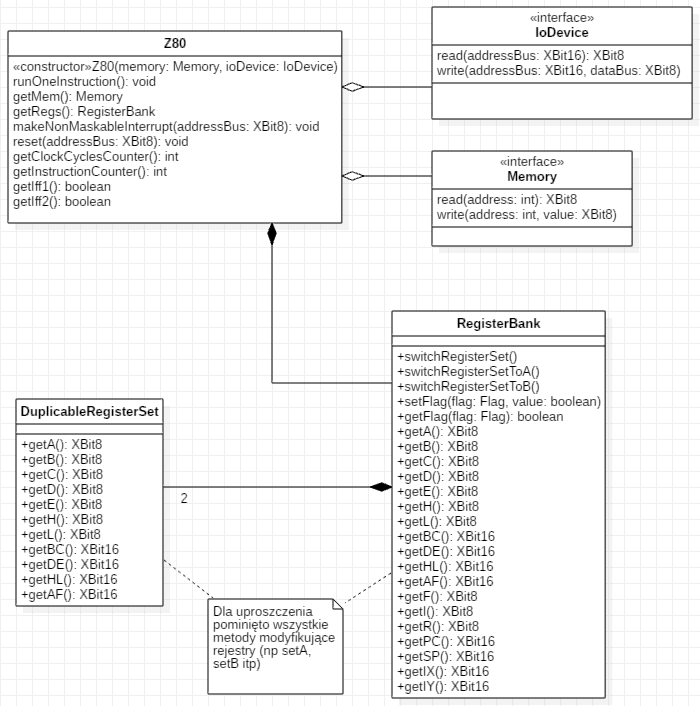
\includegraphics[width=0.9\textwidth]{z80emuCoreUml}
		\caption{Diagram hierarchii klas dla modułu z80emu{\dywiz}core}
		\label{img:z80emuCoreUml}
	\end{figure}
	
	\subsection{Łączenie z innymi projektami}
		
	Postanowiono nie uruchamiać procesu emulacji w pętli głównej tak jak w klasycznym podejściu pokazanym w kodzie \ref{listing:interpreter}. Zamiast tego udostępniono jedną metodę \emph{runOneInstruction()} która wykonuje jeden rozkaz procesora.
	
	Metody sterujące procesem emulacji (np. wywołanie przerwania, edycja rejestrów) powinny zostać wywoływane między kolejnymi wywołaniami \emph{runOneInstruction()}. Główna pętla emulacji powinna zostać zaimplementowania w module nadrzędnym, używającym \emph{z80emu{\dywiz}core}. Pozwala to na większą elastyczność modułu w łączeniu go z innymi projektami.
	
	Inną ważną decyzją projektową pozwalającą na zwiększenie elastyczności projektu, było zaprojektowanie interfejsów \emph{IoDevice} oraz \emph{Memory} i decyzja o zaimplementowaniu jedynie prostych reprezentacji klas implementujących te interfejsy.
	Aby uzasadnić powód wprowadzenia tego rozwiązania na rysunku \ref{img:z80minimalnySystemKomputerowy} przedstawiono minimalny system komputerowy oparty na procesorze Z80.
	Widać na nim, że pamięć programu (na rysunku jest to 8kb ROM) oraz podłączone urządzenie wejścia/wyjścia (na rysunku \emph{Z80-PIO}, który jest programowalnym układem wejścia/wyjścia) są osobnymi urządzeniami i mogą one być różne w zależności od systemu komputerowego. Interfejsy \emph{IoDevice} oraz \emph{Memory} pozwalają na implementację zachowania takich urządzeń, jakie są wymagane dla docelowego projektu. 
	
	
	\begin{figure}[h]
		\centering
		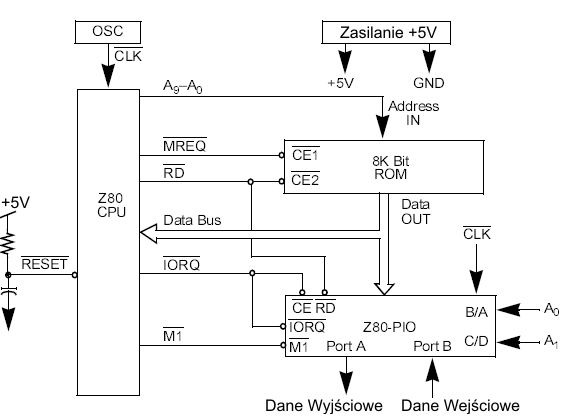
\includegraphics[width=0.6\textwidth]{z80minimalnySystemKomputerowy}
		\caption{Minimalny System Komputerowy Z80}
		\label{img:z80minimalnySystemKomputerowy}
	\end{figure}
		
	\section{Z80emu{\dywiz}gui}
	\emph{Z80emu{\dywiz}gui} to moduł realizujący interfejs użytkownika. Został on napisany z pomocą biblioteki \emph{JavaFX}. Projekt interfejsu obejmował stworzenie makiety w języku FXML zaprezentowanej na grafice \ref{img:z80Gui}. Większość interfejsów emulatorów posiada GUI złożone z wielu okien, które można dowolnie zamykać i otwierać, a każde z nich zawiera osobny moduł. Dla przykładu, w \emph{Z80 simulator IDE}, edytor pamięci, asembler lub manipulacja urządzeniami wejścia wyjścia zawarte są w osobnych oknach. 
	W projekcie \emph{Z80emu{\dywiz}gui} postanowiono stworzyć interfejs zawierający wszystkie funkcje w jednym oknie. 
	
	\begin{figure}[h]
		\centering
		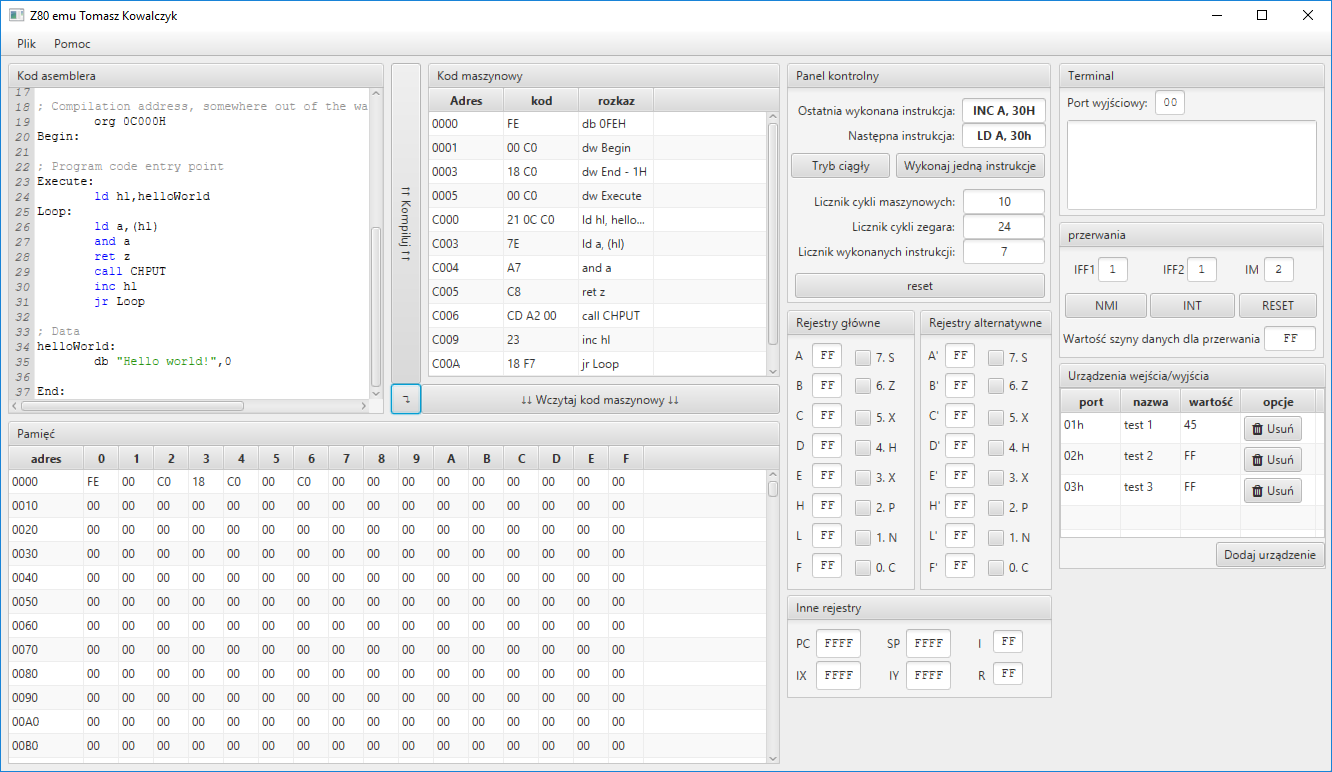
\includegraphics[width=1\textwidth]{z80Gui}
		\caption{Makieta interfejsu użytkownika}
		\label{img:z80Gui}
	\end{figure}
	 
	
	Elementy interfejsu użytkownika podzielono na dwa zbiory w celu czytelniejszego objaśnienia ich roli. Pierwszy zbiór zaprezentowany na grafice \ref{img:z80GuiPart1WithPoints} zawiera elementy związane ze sterowaniem pamięcią oraz kodem programu. Opis poszczególnych elementów umieszczonych na schemacie:
	\begin{enumerate}
		\item edytor kodu asemblera, z prostym kolorowaniem składni,
		\item widok kodu maszynowego w formie tabeli, zawierającej informacje o adresie rozkazu w pamięci, kodzie maszynowym oraz czytelnej dla człowieka nazwie instrukcji,
		\item tabela reprezentująca moduł pamięci podłączony do procesora,
		\item przycisk kompilujący kod asemblera (p. 1) do kodu maszynowego (p. 2),
		\item przycisk wczytujący kod maszynowy programu(p. 2), do pamięci procesora (p. 3),
		\item przycisk wykonujący kompilacje kodu asemblera (p. 1) a następnie wczytanie go do pamięci (p. 3).
	\end{enumerate}
	
	\begin{figure}[h]
		\centering
		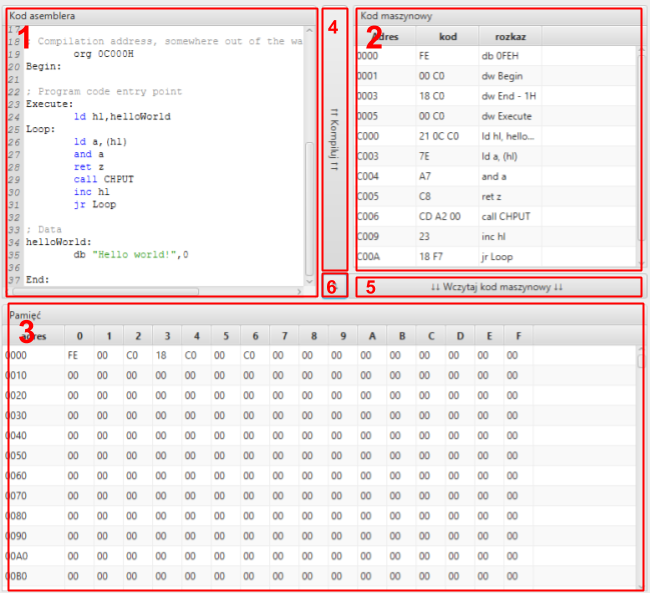
\includegraphics[width=1\textwidth]{z80GuiPart1WithPoints}
		\caption{Makieta interfejsu użytkownika z oznaczeniami. Część 1}
		\label{img:z80GuiPart1WithPoints}
	\end{figure}
	
	Drugą część interfejsu zaprezentowano na grafice \ref{img:z80GuiPart2WithPoints}. Oto opis poszczególnych elementów:
	\begin{enumerate}
		\item główny panel kontrolujący proces emulacji, przedstawiający między innymi liczbę cykli maszynowych i zegara wykonywanego programu,
		\item pola prezentujące nazwę ostatniej wykonanej i następnej w kolejce instrukcji procesora,
		\item przycisk uruchamiający emulację ciągłą (ponownie jego wybranie zatrzymuje emulacje),
		\item przycisk wykonujący pojedynczy, następny rozkaz procesora,
		\item przycisk resetujący urządzenie,
		\item widok rejestrów głównych i alternatywnych włącznie z flagami,
		\item widok rejestrów I, R, PC, SP, IX, IY,
		\item terminal wyjściowy, emulujący na stałe przypisane urządzenie,
		\item pole tekstowe, do którego wpisywany jest numer portu terminala wyjściowego, pod jakim będzie przyjmował on dane,
		\item panel grupujący elementy interfejsu odpowiedzialne za przerwania,
		\item przycisk generujący NMI (z ang. \emph{Non-Maskable Interrupt}), sygnał przerwania niemaskowanego,
		\item przycisk generujący INT (z ang. \emph{Interrupt}), sygnał maskowanego przerwania,
		\item przycisk generujący sygnał resetu,
		\item pole tekstowe zawierające 8{\dywiz}bitową wartość, jaką przyjmie szyna danych podczas zgłoszenia przerwania,
		\item tabela z listą podłączonych urządzeń wejścia/wyjścia,
		\item przycisk pozwalający na usunięcie urządzenia wejścia/wyjścia,
		\item przycisk dodający nowe urządzenie wejścia/wyjścia.
	\end{enumerate}
	
	\begin{figure}[h]
		\centering
		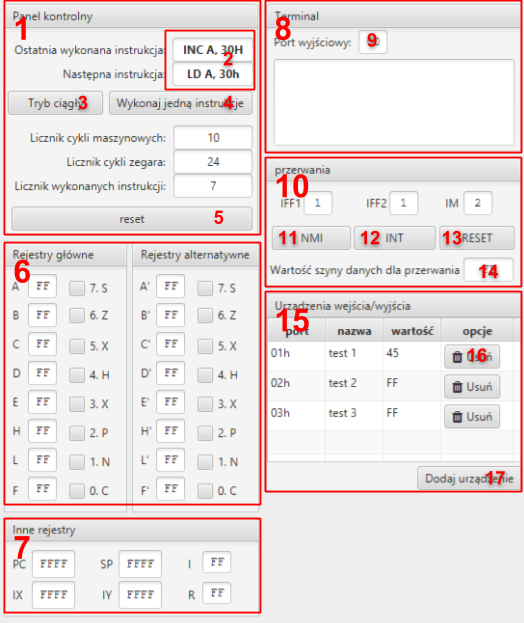
\includegraphics[width=0.8\textwidth]{z80GuiPart2WithPoints}
		\caption{Makieta interfejsu użytkownika z oznaczeniami. Część 2}
		\label{img:z80GuiPart2WithPoints}
	\end{figure}

	%tutaj o mvc
	
	W rozdziale opracowano wymagania funkcjonalne i niefunkcjonalne aplikacji. Zaprojektowano strukturę projektu podzieloną na trzy moduły. Głównym kryterium, jakie przyjęto podczas projektowania, jest możliwość ponownego użycia każdego z nich w innym projekcie emulatora. W ramach projektu stworzono także makietę interfejsu użytkownika w języku FXML.
	\chapter{Implementacja}
    W rozdziale tym przedstawiono proces implementacji projektu. Najpierw opracowano moduł \emph{XBit}, następnie \emph{Z80emu{\dywiz}core} i~na końcu \emph{Z80emu{\dywiz}gui}. Implementację każdego z~nich opisano w osobnym podrozdziale. Zaprezentowano najciekawsze fragmenty kodu źródłowego i je opisano. 

	\section{XBit}

\emph{XBit} to moduł mający za zadanie ułatwić operacje bitowe w języku Java, która interpretuje liczby całkowite w kodzie dopełnień do dwóch i nie jest możliwa interpretacja ich w naturalnym kodzie binarnym (w skrócie NKB). Z tego powodu powstał moduł \emph{XBit} implementujący taką operację. Potrafi on odczytać liczbę n{\dywiz}bitową i zwrócić jej wartość jako zmienną typu \emph{int}, interpretując ją jako bity w U2 lub NKB.


Wewnątrz obiektów reprezentujących liczby binarne, wartość przechowywana jest w~polu typu \emph{int}, które nazwano \emph{valueContainer}. Może ono przyjąć teoretycznie wartości od -2147483648 do 2147483647. Uznano jednak, że atrybut ten przechowywał będzie wartość, jaką reprezentują przechowywane bity w notacji NKB (czyli tylko wartości dodatnie). Z tego powodu wartość \emph{valueContainer} nigdy nie będzie ujemna. \newline
Zakres wartości tego pola to od 0 do $ 2^{n}-1, n<32 $ gdzie \emph{n} oznacza liczbę bitów, jaką przechowuje dany obiekt. Ponieważ typ \emph{int} przechowywany jest w czterech bajtach i interpretowany jest przez język Java w notacji U2, maksymalnie może przechować wartość 2 147 483 647. Dla wartości interpretowanej w NKB na czterech bajtach jest to \newline $2^{32}-1 =$ 4 294 967 296. Jest to więcej niż typ \emph{int} może zawierać, dlatego maksymalna możliwa binarna reprezentacja, jaka może zostać zapisana w podobny sposób, to liczba przechowywana na 31 bitach.

Jeśli obiekt \emph{XBit8} będzie przechowywał liczbę binarną 11111111 (czyli odczytując w~NKB to decymalne 255, a w U2 decymalnie -1). Wartość jego pola \emph{valueContainer} będzie wynosić w~kodzie binarnym
00000000 00000000 00000000 11111111. (czyli odczytując zarówno w NKB, jak i w U2 będzie to 255). Niestety nadmiarowość bitów jest w tym rozwiązaniu wymagana, ponieważ liczba w kodzie U2, której najbardziej znaczący bit ma wartość $1$, jest ujemna. 

Podsumowując, \emph{XBit} wykorzystuje fakt takiego samego zapisu liczb dodatnich w U2 i NKB, jeśli tylko będą one zapisane na większej liczbie bitów niż wymagana.


\subsection{Implementacja klasy \emph{XBit}}
\emph{XBit} to klasa abstrakcyjna zawierająca wspólne elementy dla klas \emph{XBit8} i \emph{XBit16} oraz, ewentualnych klas dziedziczących.W~tym podrozdziale zawarto opis najbardziej istotnych metod tej klasy.

\subsubsection{boolean getBit(int index)}

\begin{listing}[h]
	\inputminted{java}{listings/xbit/xbitMethodGetBit.java}
	\caption{Metoda boolean getBit(int index)}
	\label{listing:xbitMethodGetBit}
\end{listing}
Na listingu \ref{listing:xbitMethodGetBit} zaprezentowano metodę \emph{getBit} zwracającą wartość bitu na pozycji o~numerze przekazanym w parametrze. W linii nr 2 sprawdzana jest poprawność parametru \emph{index}. Jeśli jest on niepoprawny, w linii nr 3 wyrzucany jest wyjątek \emph{NumberFormatException}. W linii nr 5 metoda wykonuje przesunięcie bitowe pola \emph{valueContainer} o~podany index. Ponieważ wynikiem jest liczba o typie \emph{int}, wykonywana zostaje koniunkcja bitowa z maską o wartości 1. Na końcu wynik operacji jest przekształcany z typu \emph{int} na \emph{boolean} i zwracany.


\subsubsection{setBit(int index, boolean value)}
\begin{listing}[h]
	\inputminted{java}{listings/xbit/xbitMethodSetBit.java}
	\caption{Metoda TSelf setBit(int index, boolean value)}
	\label{listing:xbitMethodSetBit}
\end{listing}	
Listing \ref{listing:xbitMethodSetBit} prezentuje metodę nadającą bitowi o określonej pozycji, zadaną wartość, a~następnie zwracającą nowy zmodyfikowany obiekt. Typ \emph{TSelf} zwracanej wartości to typ generyczny reprezentujący docelową liczbę n-bitową. W linii nr 2 metoda tworzy maskę bitową, wykonując przesunięcie bitowe na liczbie 1 o wartość parametru \emph{index}, czyli maska będzie posiadała tylko jeden bit ustawiony na wartość $1$, i będzie to bit o~pozycji z~parametru. W liniach 5 i 7 metoda wykonuje operacje bitowe mające na celu zmianę bitu na 1 lub 0 w zależności od parametru \emph{value}:
\begin{itemize}  
	\item dla \emph{value} równego 1 wykonywane są instrukcje zawarte w~linii nr~5. Najpierw pobierana jest obecna wartość obiektu i wykonana alternatywa bitowa  na niej i na wcześniej zbudowanej masce. Metoda przypisuje wynik do zmiennej \emph{newValue} będącej buforem,
	\item dla \emph{value} równego 0 metoda wykonuje instrukcje zawartą w linii nr~7. Nowa wartość uzyskiwana jest przez koniunkcje bitową aktualnej wartości oraz negacji maski. 
\end{itemize} 

\subsubsection{int getValueOfBits(int startIndexBit, int stopIndexBit)}
\begin{listing}[h]
	\inputminted{java}{listings/xbit/getValueOfBits.java}
	\caption{Metoda int getValueOfBits(int startIndexBit, int stopIndexBit)}
	\label{listing:getValueOfBits}
\end{listing}
Listing \ref{listing:getValueOfBits} przedstawia metodę zwracającą fragment wartości binarnej, od pozycji określonej przez argument \emph{startIndexBit}. do \emph{stopIndexBit}, włącznie.

W liniach 2 i 3 sprawdzana jest poprawność argumentów i ewentualnie zostaje wyrzucony wyjątek.  W linii 6 tworzony jest bufor, wykonując przesunięcie bitowe w prawo na wartości obiektu, o wartość parametru \emph{stopIndexBit}. Dzięki tej operacji pozbyto się zbędnych bitów z wartości obiektu po prawej stronie. Następnym krokiem jest pozbycie się bitów po lewej stronie. W tym celu, w linii nr 7 wykonywana jest maska bitowa wypełniona taką liczbą jedynek, jak liczba bitów docelowej wartości. Aby ją wykonać, wykonujemy przesunięcie bitowe w lewo na maksymalnej liczbie, jaką może przyjąć typ \emph{int} (w zapisie binarnym 01111111 11111111 11111111 11111111) o liczbę bitów wartości docelowej - 1. Następnie wykonano negację bitową. Bitów po lewej stronie pozbyto się za pomocą operacji iloczynu bitowego na uzyskanej masce i buforze.

\subsubsection{Inne metody}
Klasa \emph{XBit} posiada inne metody, zbyt proste w swojej budowie, aby były warte dokładniejszego opisywania. Zostaną one jedynie wymienione w celu lepszego zobrazowania wszystkich możliwości.
\begin{itemize}  
	\item \emph{public abstract short getSize()} - abstrakcyjna metoda zwracająca liczbę bitów jakie przechowuje docelowa liczba,
	\item \emph{public abstract int getMinSignedValue()} - zwraca minimalną liczbę ze znakiem jaka może być przechowywana w obiekcie,
	\item \emph{public abstract int getMaxSignedValue()} - zwraca maksymalną liczbę ze znakiem jaka może być przechowywana w obiekcie,
	\item \emph{public int getMinUnsignedValue()} - zwraca minimalną liczbę bez znaku jaka może być przechowywana w obiekcie (czyli zawsze przyjmuje wartość 0),
	\item \emph{public abstract int getMaxUnsignedValue()} - zwraca maksymalną liczbę bez znaku jaka może być przechowywana w obiekcie,
	\item \emph{public boolean isNegative()} - zwraca wartość bitu o największej pozycji, który w kodowaniu U2 decyduje czy liczba jest mniejsza od zera,
	\item \emph{public int getSignedValue()} - zwraca wartość w kodowaniu U2,
	\item \emph{public int getUnsignedValue()} - zwraca wartość w kodowaniu NKB.
\end{itemize}

\subsection{Implementacja klasy \emph{XBit8}}
Klasa \emph{XBit8} dziedziczy po abstrakcyjnej klasie \emph{XBit}, która została zbudowana w taki sposób, aby klasy po niej dziedziczące były jak najmniejsze. Metody, które należą do \emph{XBit8} i nie zostały odziedziczone. Nie są one na tyle skomplikowane, aby warto było je bardziej szczegółowo opisywać, z tego powodu zostaną wymienione i krótko opisane.
\begin{itemize}  
	\item \emph{public static XBit8 valueOfUnsigned(int value)} - tworzy nowy obiekt o wartości bez znaku,
	\item \emph{public static XBit8 valueOfSigned(int value)} - tworzy nowy obiekt o wartości ze znakiem,
	\item \emph{public static XBit8 valueOfBooleanArray(boolean[] values)} - tworzy nowy obiekt na podstawie tablicy elementów o typie \emph{boolean}.
\end{itemize}

\subsection{Implementacja klasy XBit16}
\emph{XBit16} to klasa reprezentująca liczbę 16 bitową. Dziedziczy ona po \emph{XBit}. Dzięki temu nie musi implementować najbardziej podstawowych metod. 


\subsubsection{public static XBit16 valueOfHighAndLowInBigEndian(XBit8 high, XBit8 low)}
\begin{listing}[h]
	\inputminted{java}{listings/xbit/valueOfHighAndLowInBigEndian.java}
	\caption{Metoda XBit16 valueOfHighAndLowInBigEndian(XBit8 high, XBit8 low)}
	\label{listing:valueOfHighAndLowInBigEndian}
\end{listing}
Listingu \ref{listing:valueOfHighAndLowInBigEndian} przedstawia implementację metody \emph{valueOfHighAndLowInBigEndian} tworzącej liczbę 16{\dywiz}bitową w formacie zapisu \emph{big endian} (najbardziej znaczący bajt umieszczony jest jako pierwszy). Przyjmuje ona jako parametry dwie liczby 8{\dywiz}bitowe o nazwach \emph{high} i \emph{low}. 
Metoda tworzy obiekt klasy \emph{ByteBuffer} należącej do standardowej biblioteki języka Java i konfiguruje ją, aby przechowywała dane w formacie \emph{big endian} (linia nr 3). 
Następne linie prezentują operacje dodania do bufora kolejno starszego (linia nr 4) i~młodszego  bajtu (linia nr 5). Na koniec wykonano metodę \emph{getShort()} zwracającą docelową liczbę i na jej podstawie tworzona jest reprezentacja klasy \emph{XBit16}.

\subsubsection{public static XBit16 valueOfHighAndLowInLittleEndian(XBit8 high, XBit8 low)}
\begin{listing}[h]
	\inputminted{java}{listings/xbit/valueOfHighAndLowInLittleEndian.java}
	\caption{Metoda XBit16 valueOfHighAndLowInLittleEndian(XBit8 high, XBit8 low)}
	\label{listing:valueOfHighAndLowInLittleEndian}
\end{listing}
W listingu \ref{listing:valueOfHighAndLowInLittleEndian} zaprezentowano metodę tworzącą liczbę 16{\dywiz}bitową w formacie zapisu \emph{little endian}, czyli najbardziej znaczący bajt umieszczony jest jako ostatni.
Implementacja metody jest dosyć prosta, wykonuje ona metodę \emph{valueOfHighAndLowInBigEndian()} z~zamienioną kolejnością parametrów.


\subsubsection{Inne metody}
Klasa \emph{XBit16} zawiera także metody, które są zbyt proste w implementacji aby warto było je opisywać pojedynczo:
\begin{itemize}  
	\item \emph{public static XBit16 valueOfUnsigned(int value)} - tworzy nowy obiekt o wartości bez znaku,
	\item \emph{public static XBit16 valueOfSigned(int value)} - tworzy nowy obiekt o wartości ze znakiem.
\end{itemize}


\subsection{Implementacja klasy XbitUtils}
\emph{XbitUtils} to klasa implementująca operacje arytmetyczne i bitowe na obiektach \emph{XBit8} i~\emph{XBit16}. Posiada ona dwie klasy wewnętrzne, \emph{Arithmetic8bitResult}  oraz \newline\emph{Arithmetic16bitResult} reprezentujące wynik operacji arytmetycznych i zawierające informacje o wystąpieniu przeniesienia i przepełnienia. Klasy te zaprezentowano w listingach \ref{listing:arithmetic8bitResult} oraz \ref{listing:arithmetic16bitResult}.

\begin{listing}[h]
	\inputminted{java}{listings/xbit/arithmetic8bitResult.java}
	\caption{Klasa Arithmetic8bitResult}
	\label{listing:arithmetic8bitResult}
\end{listing}

\begin{listing}[h]
	\inputminted{java}{listings/xbit/arithmetic16bitResult.java}
	\caption{Klasa Arithmetic16bitResult}
	\label{listing:arithmetic16bitResult}
\end{listing}

\subsubsection{public static XBit8 incrementBy(XBit8 value, int incrementer)}
\begin{listing}[h]
	\inputminted{java}{listings/xbit/incrementBy.java}
	\caption{Metoda XBit8 incrementBy(XBit8 value, int incrementer)}
	\label{listing:incrementBy}
\end{listing}
Listing \ref{listing:incrementBy} prezentuje metodę zwiększającą liczbę 8{\dywiz}bitową o daną wartość. Aby wykonać operację, metoda konwertuje parametr \emph{value} na liczbę typu \emph{int} (linia nr 2) i dodaje wartość parametru \emph{incrementer} (linia nr 3). Następnie w linii nr 4 wykonuje operacje iloczynu bitowego na uzyskanej nowej wartości oraz masce bitowej reprezentującej największą możliwą wartość, jaką może przechowywać liczba 8{\dywiz}bitowa (celem tej operacji jest niedopuszczenie do sytuacji, w której wynik operacji nie mieści się na ośmiu bitach). Na koniec tworzona jest i zwracana instancja klasy \emph{XBit8}. 

Zasada działania metody \emph{XBit16 incrementBy(XBit16 value, int incrementer)} jest podobna, dlatego jej opis zostanie pominięty. 

\subsection{public static XBit8 negativeOf(XBit8 value)}
\begin{listing}[h]
	\inputminted{java}{listings/xbit/negativeOf.java}
	\caption{Metoda XBit8 negativeOf(XBit8 value)}
	\label{listing:negativeOf}
\end{listing}
Funkcja tworząca liczbę o~przeciwnym znaku do podanej została zaprezentowana w~listingu \ref{listing:negativeOf}. Operacja ta polega na wykonaniu iloczynu bitowego na negacji bitowej danej wartości oraz liczbie 255. Ma to na celu niedopuszczenie do sytuacji, w której wartość bufora będzie większa niż 255, a więc nie będzie mogła się zmieścić na ośmiu bitach.
Następnie wykonany wynik zostaje zwiększony o jeden. 

Zasada działania metody \emph{XBit16 negativeOf(XBit16 value)} jest taka sama. Jedyną różnicą jest operacja iloczynu bitowego, którą wykonujemy nie na liczbie 255 a 65535.

\subsection{public static Arithmetic8bitResult addTwo8bits(XBit8 value1, XBit8 value2)}
\begin{listing}[h]
	\inputminted{java}{listings/xbit/addTwo8bits.java}
	\caption{Metoda Arithmetic8bitResult addTwo8bits(XBit8 value1, XBit8 value2)}
	\label{listing:addTwo8bits}
\end{listing}
Listing \ref{listing:addTwo8bits} prezentuje metodę realizującą dodawanie dwóch liczb 8-bitowych. Wynikiem jej działania jest obiekt klasy \emph{Arithmetic8bitResult} przechowujący wynik operacji i flagi przepełnienia lub przeniesienia. 

W linii nr 3 metoda wykonuje operacje dodawania. W linii nr 4 umieszczono sprawdzenie, czy nastąpiło przepełnienie, a linia nr 5 ustawia flagę. Linia nr 7 wykonuje ,,obcięcie" bitów w przypadku, gdy wynik nie będzie w stanie zmieścić się w liczbie 8{\dywiz}bitowej.

Linie 9 i 10 zawierają operację ustawiającą flagę przepełnienia według\newline trzech zasad \cite{overflowRules}:
\begin{enumerate}
	\item jeśli suma dwóch liczb dodatnich daje wynik ujemny, to znaczy, że wystąpiło przepełnienie,
	\item jeśli suma dwóch liczb ujemnych daje wynik dodatni, to również oznaca wystąpienie przepełnienia,
	\item w każdym innym przypadku przepełnienie nie wystąpiło.
\end{enumerate}
Zakłada się, że najbardziej znaczący bit jest bitem znaku.

Prezentacja metody realizującej dodawanie dwóch liczb 16{\dywiz}bitowych została pominięta, ponieważ operacja ta jest przeprowadzana na tej samej zasadzie co 8{\dywiz}bitowa.

\subsection{public static Arithmetic8bitResult subTwo8bits(XBit8 value1, XBit8 value2)}
\begin{listing}[h]
	\inputminted{java}{listings/xbit/subTwo8bits.java}
	\caption{Metoda Arithmetic8bitResult subTwo8bits(XBit8 value1, XBit8 value2)}
	\label{listing:subTwo8bits}
\end{listing}
W listingu \ref{listing:subTwo8bits} zaprezentowano metodę realizującą odejmowanie jednej liczby 8{\dywiz}bitowej, od drugiej. Metoda wykorzystuje regułę 
$ a - b = a+(-b) $ według której odejmowanie dwóch liczb można zastąpić dodawaniem, negując drugi składnik odejmowania. 
Metoda realizująca odejmowanie dwóch liczb 16{\dywiz}bitowych działa w analogiczny sposób.

\subsection{public static XBit8 not8bit(XBit8 value)}
\begin{listing}[h]
	\inputminted{java}{listings/xbit/not8bit.java}
	\caption{Metoda XBit8 not8bit(XBit8 value)}
	\label{listing:not8bit}
\end{listing}
Metoda \emph{not8bit(XBit8 value)} zaprezentowana w listingu \ref{listing:not8bit} wykonuje negację bitową na liczbie 8{\dywiz}bitowej. Operacja wykonywana jest za pomocą standardowego operatora negacji bitowej języka Java (znak tyldy górnej ,,\~{}"). Dodatkową wykonywaną operacją jest iloczyn bitowy z liczbą 255, mający za zadanie wyzerowanie bitów starszych od ósmego. Wersja metody dla liczb 16{\dywiz}bitowych jest analogiczna.

\subsection{public static XBit8 and8bit(XBit8 value1, XBit8 value2)}
\begin{listing}[h]
	\inputminted{java}{listings/xbit/and8bit.java}
	\caption{Metoda XBit8 and8bit(XBit8 value1, XBit8 value2)}
	\label{listing:and8bit}
\end{listing}
Listing \ref{listing:and8bit} prezentuje metodę wykonującą operację sumy logicznej dwóch liczbe \mbox{8{\dywiz}bitowych} (linia nr 3). Linia nr 4 zawiera operację wyzerowania bitów starszych od ósmego dla wyniku, aby mieścił się on w ośmiu bitach. Wersja metody dla liczb \mbox{16{\dywiz}bitowych} działa analogicznie.

\subsection{Metody wykonujące sumę bitową i różnice symetryczną}
Implementacje metod:
\begin{itemize}  
	\item \emph{public static XBit8 or8bit(XBit8 value1, XBit8 value2)},
	\item \emph{public static XBit16 or16bit(XBit16 value1, XBit16 value2)},
	\item \emph{public static XBit8 xor8bit(XBit8 value1, XBit8 value2)},
	\item \emph{public static XBit16 xor16bit(XBit16 value1, XBit16 value2)},
	\item \emph{public static XBit8 shift8bit(XBit8 value1, int position)},
	\item \emph{public static XBit8 shift16bit(XBit8 value1, int position)}.
\end{itemize}
są analogicznie do metody and8bit(XBit8 value1, XBit8 value2). Operacje bitowe wykonywane są za pomocą mechanizmów wbudowanych w język Java, a nadmiar bitów zostaje obcięty.
	\section{Z80emu-core}
Z80emu-core to moduł mający za zadanie wykonać proces emulacji. Używa on do swojego działania bibliotekę XBit.

@todo tutaj podział na pakiety

\subsection{obiekt klasy Z80}

\subsection{opis registerbank}

\subsection{opis flagmanager}

\subsection{opis memory}

\subsection{opis io}

\subsection{InstructionDecoder i instructionContainer}

\subsection{opis instrukcje}

\subsection{opis helpery do instrukcji}

	\section{Z80emu{\dywiz}gui}

Moduł \emph{Z80emu{\dywiz}gui} implementuje interfejs użytkownika zaprezentowany na rysunku nr \ref{img:z80Gui}. Został on napisany z pomocą biblioteki \emph{JavaFX}. Największą jej zaletą w porównaniu do poprzedniczki, którą była biblioteka \emph{Swing}, jest możliwość definiowania widoku aplikacji za pomocą języków XML i CSS. Projektowanie interfejsu w \emph{JavaFx} przypomina nieco tworzenie strony WWW.

Kod źródłowy implementujący interfejs użytkownika został podzielony na pakiety, których strukturę przedstawiono na rysunku \ref{img:z80EmuGuiPackage}. Postanowiono podzielić pliki zgodnie ze wzorcem \emph{Model-View-Controller}, który dzieli aplikacje na trzy główne części. Każda z~nich ma swoją reprezentację w module jako oddzielna paczka:
\begin{itemize}
    \item \emph{model} - implementuje logikę biznesową. W tym przypadku, między innymi zarządza procesem asemblacji i emulacji.
    \item \emph{View} - opisuje widok aplikacji. W projektach zbudowanych za pomocą \emph{javaFx} są to pliki XML i CSS. Oprócz nich mogą też być pliki języka Java, odpowiedzialne za prezentację danych. W opisywanym projekcie są to np. klasy, których zadaniem jest kolorowanie składni w edytorze kodu asemblera, tworzenie okien dialogowych lub system pomocy.
    \item \emph{controller} - zadaniem kontrolera jest przetworzenie informacji od użytkownika, by na jej podstawie wywoływać metody modelu i aktualizować widok. W projekcie każda część interfejsu posiada osobny kontroler (dla przykładu, osobne kontrolery zajmują się pamięcią programu, przerwaniami, i edytorem kodu asemblera).
\end{itemize}

\begin{figure}[h]
		\centering
		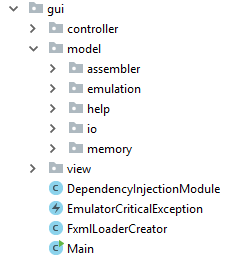
\includegraphics[width=0.4\textwidth]{z80EmuGuiPackage}
		\caption{Podział na pakiety modułu z80emu{\dywiz}gui}
		\label{img:z80EmuGuiPackage}
\end{figure}



\subsection{Wstrzykiwanie zależności za pomocą biblioteki \emph{Guice}}
Wstrzykiwanie zależności (z ang. \emph{Dependency Injection}) to technika programowania, której głównym założeniem jest przekazywanie gotowych skonfigurowanych już obiektów do innych (wstrzykiwanie ich), które ich wymagają. Moduł interfejsu użytkownika posiada wiele współpracujących ze sobą  klas. Zarządzanie nimi stało się z czasem uciążliwe. Problem postanowiono rozwiązać z pomocą biblioteki \emph{Guice}, która implementuje technikę wstrzykiwania zależności.

Aby opisać problem, należy przedstawić, z jakich elementów zostały zbudowane kontrolery w projekcie. Fragment jednego z nich został zaprezentowany w listingu \ref{listing:z80DiCOntrollerExample}. Kontroler ten jest zależny od modelu (linie nr 3-5) oraz posiada obiekty wstrzykiwane przez bibliotekę graficzną na podstawie plików FXML (linie nr 7 i 8). Zatem należało użyć biblioteki \emph{Guice} nie wprowadzając przy tym konfliktów z \emph{JavaFX}.

\begin{listing}[h]
	\inputminted{java}{listings/z80emu-gui/DiControllerExample.java}
	\caption{Zależności klasy \emph{MemoryController}}
	\label{listing:z80DiCOntrollerExample}
\end{listing}

Połączono \emph{JavaFx} i \emph{Guice} w następujący sposób. Interfejs biblioteki graficznej posiada metodę \emph{setControllerFactory(Callback<Class<?>, Object> controllerFactory)}, potrafiącą podmienić domyślną fabrykę kontrolerów. Jako jej parametr przekazano metodę biblioteki \emph{Guice} \emph{<T> T getInstance(Class<T> type)}, która zwraca instancję danego obiektu. Dzięki takiemu rozwiązaniu, kontrolery mają możliwość używania wszystkich adnotacji ułatwiających wstrzykiwanie do nich zależności (a nawet innych kontrolerów) i jednocześnie są udekorowane w~obiekty biblioteki graficznej.

\subsection{Integracja z projektem Z80emu{\dywiz}core}

\begin{listing}[h]
	\inputminted{java}{listings/z80emu-gui/EmulatorThread.java}
	\caption{Klasa \emph{EmulatorThread} realizująca emulację w trybie ciągłym}
	\label{listing:emulatorThread}
\end{listing}

\emph{Z80emu{\dywiz}gui} używa do emulacji modułu \emph{Z80emu{\dywiz}core}, który zawiera metodę \emph{runOneInstruction} wykonującą kolejną instrukcję CPU. Pomiędzy jej kolejnymi wywołaniami powinny zostać zgłoszone przerwania lub odczytane wartości rejestrów, pamięci i flag. Aby umożliwić to zarówno w trybie ciągłym, jak i krokowym wymagane było umieszczenie emulacji w osobnym wątku.

W tym celu wykonano klasę \emph{EmulatorThread}, którą pokazano w listingu \ref{listing:emulatorThread}. Użytkownik może uruchomić i zatrzymać emulację w dowolnym momencie za pomocą publicznych metod \emph{pause} i \emph{unPause}.

Metoda \emph{pause}, która docelowo zostaje wywoływana z innego wątku, zmienia wartość pola \emph{pause} typu \emph{boolean} na \emph{false}.  W głównej pętli emulacji sprawdzany jest warunek \emph{if(pause) \{lock.wait(); pause = false;\}}. Jeśli jest on spełniony, to wątek jest wprowadzany w stan oczekiwania.

Metoda \emph{unPause}, która także wywoływana jest z innego wątku, odblokowuje wątek, i~pozwala wznowić emulację.

% pomysły co mogło by się znaleźć w tym dziale: 
% - o wątkach, jak zaimplementowałem debugowanie ciągłe

% - podział na kontrolery, że jest wiele kontrolerów a nie jeden główny
% - opisać, jak podpiąłem biblioteke asemblującą, wspomnieć że to nie jest moje dzieło
% - ?? opisać jak działają przerwania
% - 
% - w jaki sposób zaimplementowano wiki, że jest to rekurencja itp. Wspomnieć że pliki jar nie mają struktury katalogów, i nie da się w nich wylistować listy plików w danym katalogu, dlatego tak to skomplikowałem
% - info co zostało niepodpięte pod gui, np przerwania


	
	Implementacja przebiegła zgodnie z założonym projektem aplikacji. Stosunkowo najbardziej czasochłonną częścią implementacji, było opracowanie klas modułu \emph{Z80emu-core}, odpowiedzialnych za realizowanie rozkazów procesora. Spowodowane to było głównie ich ilością (158 instrukcji). Moduł \emph{XBit} spełnił swoje zadanie i znacznie uprościł kod źródłowy emulatora. 
	
	
	
		
	\chapter{Testy}
	Ten rozdział zawiera opis metodologii przeprowadzonych testów oraz komentuje ich wyniki. Nawet niewielkie defekty w~kodzie emulatora mogą spowodować błędne działanie programów przeznaczonych dla procesora Zilog Z80 lub wręcz uniemożliwić ich wykonanie. Dlatego dla każdej metody implementującej rozkaz procesora został opracowany co najmniej jeden test jednostkowy. Testy jednostkowe zaimplementowane przy pomocy biblioteki JUnit. Dodatkowo wykonano także testy manualne, polegające na wykonaniu programów na opracowanym emulatorze i~\emph{Z80 Simulator IDE}, a~następnie porównaniu ich wyników.
	
	\section{Testy jednostkowe}
	Testy jednostkowe to programy, które mają za zadanie weryfikować działanie określonego fragmentu testowanego oprogramowania. W omawianej aplikacji zostały użyte celem sprawdzenia czy rozkazy procesora są poprawnie emulowane.
	
	Kod testujący powstał przed napisaniem implementacji danej funkcji. Takie podejście nazywane jest \emph{Test{\dywiz}driven development}. Programista najpierw określa wymagania, jakie powinna spełniać dana metoda, a następnie pisze jej implementacje. Pozwala to na opracowanie oprogramowania o~lepszej jakości, ponieważ informatyk pisząc testy, ustala wymagania dla danego fragmentu kodu, które potem stara się spełnić\cite{tdd}.
	
	\begin{listing}[H]
		\inputminted{Java}{listings/exampleTest.java}
		\caption{Test jednostkowy instrukcji LoadAFromITest.java}
		\label{listing:LoadAFromITest}
	\end{listing}
	
	Na listingu \ref{listing:LoadAFromITest} zaprezentowano test instrukcji wczytującej zawartość rejestru \emph{I} do rejestru \emph{A} (rozkaz \emph{LD A, I}). Przedstawiony przykład pokazuje, że prosta z pozoru operacja, jaką jest pobranie wartości jednego rejestru i przeniesienie go do innego, wymaga złożonych testów.	Test sprawdza poprawność wartości umieszczonej w rejestrze docelowym, flag procesora, licznika cykli i rejestru \emph{PC} za pomocą metody \emph{assertEquals}.
	
	\section{Testy manualne}
	Testy manualne polegają na weryfikowaniu poprawności działania oprogramowania, przez człowieka, bez udziału narzędzi automatyzujących. Przeprowadza się je między innymi na poziomie interfejsu użytkownika aplikacji. Wykonano emulację przykładowych programów napisanych w~asemblerze na opracowanym oprogramowaniu i~emulatorze \emph{Z80 Simulator IDE}, a następnie porównano wyniki działania w postaci stanu rejestrów, flag i pamięci. Kody źródłowe programów zastosowanych do testów, zaczerpnięto z książki Rodney'a Zaks'a \emph{Programming the Z80}\cite{programming_the_z80}.
	
	Listing \ref{listing:findingTheLargestElementOfTable} zawiera program użyty w jednym z testów manualnych, wskazujący w tablicy liczb, element o~największej wartości. Wymaga on wprowadzenia do pamięci, począwszy od adresu \emph{30h} tablicy, której pierwszy bajt zawiera liczbę przechowywanych elementów.
	Kod programu wprowadzono zarówno do pamięci stworzonego w~ramach pracy emulatora, jak i \emph{Z80 Simulator IDE}, razem z tablicą elementów: \emph{03h}, \emph{10h}, \emph{40h}, \emph{20h}. 
	
	% przykładowy kod testujący to: http://www.z80.info/zip/programming_the_z80_3rd_edition.pdf str: 526 FINDING THE LARGEST ELEMENT OF A TABLE
	\begin{listing}[h]
		\inputminted{asm}{listings/findingTheLargestElementOfTable.asm}
		\caption{Program wskazujący największą wartość w tablicy}
		\label{listing:findingTheLargestElementOfTable}
	\end{listing}   
	  \newpage
	Zrzuty ekranów \ref{img:manualTest1Memory} i \ref{img:manualTest1MemoryIDE} prezentują pamięć obu emulatorów po wykonaniu programu. 
	Komórki o adresach \emph{50h-51h} przechowują adres, pod którym znajduje się znaleziona największa wartość w~tablicy. Oba emulatory wskazały na liczbę 40, więc poprawnie wykonały program. 
	
	\begin{figure}[h]
    		\centering
    		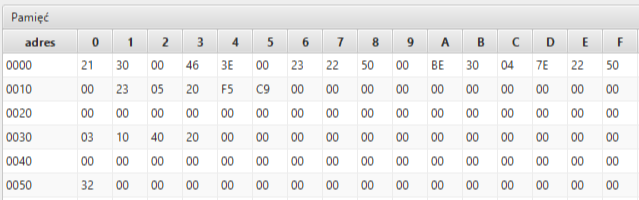
\includegraphics[width=1.0\textwidth]{manualTests/manualTest1Memory}
    		\caption{Zrzut ekranu aplikacji \emph{Z80Emu} (opracowany emulator) prezentujący pamięć procesora po wykonaniu testowego programu }
    		\label{img:manualTest1Memory}
    \end{figure}
    
    \begin{figure}[h]
    		\centering
    		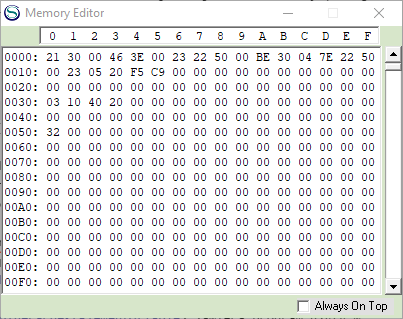
\includegraphics[width=0.6\textwidth]{manualTests/manualTest1MemoryIDE}
    		\caption{Zrzut ekranu aplikacji \emph{Z80 Simulator IDE} prezentujący pamięć procesora po wykonaniu testowego programu}
    		\label{img:manualTest1MemoryIDE}
    \end{figure}
    
    Zrzuty ekranu \ref{img:testManualnyRejestry} przedstawiają stan rejestrów, flag i liczników po wykonaniu programu. Można zauważyć, że niektóre rejestry w emulatorze \emph{Z80Emu} przyjmują wartość \emph{00h}, natomiast w \emph{ Z80 Simulator IDE} wartość \emph{FFh}. Są to rejestry, na które testowy program  nie wpływa. Nie jest to błąd. Domyślnie rejestry w Zilog-u Z80 mają wartość nieokreśloną i emulatory mogą przyjąć dowolną. Oprócz nich wszystkie wartości rejestrów, flag oraz liczników zgadzają się między obydwoma aplikacjami.
    
    \newpage
    Testowanie aplikacji było czasochłonnym i ważnym etapem przez specyfikę projektu. Emulator to program wrażliwy na błędy, i wymagane jest dokładne zweryfikowanie działania wszystkich emulowanych rozkazów procesora.
    
    \begin{figure}[h]
    		\centering
    		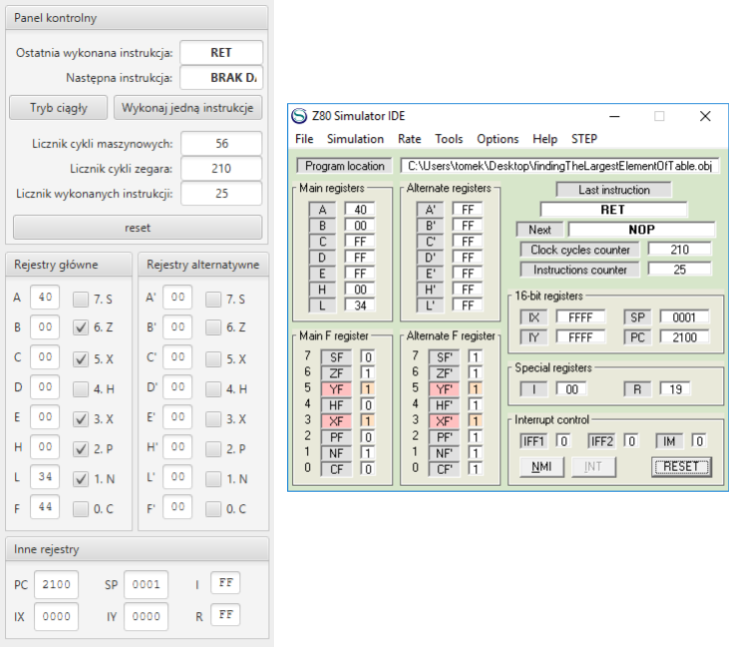
\includegraphics[width=1.0\textwidth]{manualTests/testManualnyRejestry}
    		\caption{Zrzut ekranu aplikacji \emph{Z80Emu} (po lewej) i \emph{Z80 Simulator IDE} (po prawej) prezentujący rejestry procesora po wykonaniu testowego programu}
    		\label{img:testManualnyRejestry}
    \end{figure}

    
    
    
    
    	
	\chapter{Uwagi i wnioski}

      Wynikiem realizacji pracy jest aplikacja pozwalająca na emulację procesora Zilog~Z80. Z celów zawartych w zadaniu na pracę dyplomową zrealizowano wszystkie, oprócz emulacji wewnętrznych magistrali procesora. Problem okazał się zbyt złożony i czasochłonny bez dostępu do dokumentacji opisującej wewnętrzną budowę procesora, której firma \emph{Zilog} nie upublicznia.
      
      Opisany w pracy emulator spośród innych podobnych rozwiązań wyróżnia się możliwością uruchomienia na wielu platformach systemowych, dzięki użyciu języka Java oraz czytelnym kodem źródłowym podzielonym na moduły, z~których każdy może zostać ponownie użyty w innym projekcie.
      
      Podczas pracy nad aplikacją napotkano dwa główne problemy. Jednym z nich, jest brak w~języku Java typu prostego przeznaczonego wyłącznie dla liczb naturalnych (ang.~\emph{unsigned}). Rozwiązano go tworząc własną implementację liczb w bibliotece Xbit. Drugim, poważniejszym problemem okazała się wrażliwość procesu emulacji na błędy. Nawet niewielkie nieprawidłowości w wykonywanych instrukcjach procesora, powodują nieprawidłowe działanie emulowanego programu. Ten problem rozwiązano testami jednostkowymi opracowanymi dla wszystkich instrukcji procesora.
      
      Każdy moduł aplikacji można rozwijać niezależnie. Wydajność biblioteki \emph{XBit} może zostać zwiększona poprzez zmianę kontenera przechowującego wartość liczby, który jest typu \emph{int}, na obiekt klasy \emph{ByteBuffer} która jest standardowym elementem języka Java.
      
      W module \emph{Z80emu{\dywiz}core} można zaimplementować \emph{debugger}, który dla trybu ciągłego emulacji zatrzymywałby wykonywany program w określonym miejscu.
      
      W \emph{Z80emu{\dywiz}gui} elementem, który mógłby zostać w przyszłości zaimplementowany i~usprawniłby obsługę programu przez osoby dopiero uczące się zasad działania procesorów, jest wbudowany w aplikację system pomocy. Zawierałby on informacje o rozkazach, rejestrach, przerwaniach i zasadach działania procesora, które można uzyskać z ogólnodostępnych źródeł. Użytkownik mógłby kliknąć tekst z podpisem konkretnego elementu interfejsu emulatora, o którym chciałby się dowiedzieć więcej, a aplikacja przekierowałaby go do odpowiedniej informacji w systemie pomocy. Dodatkowo wersja anglojęzyczna interfejsu pozwoliłaby na dotarcie do większej liczby użytkowników.
    
    \addcontentsline{toc}{chapter}{Bibliografia}
	\begin{flushleft}
	\begin{thebibliography}{99}
	    \bibitem{howDoIWriteAnEmulator}
		Boris D., \emph{How Do I Write an Emulator?} (online),
		https://www.atarihq.com/danb/files/emu\_vol1.txt (10 grudnia 2018).
	
	    \bibitem{emulationOrSimulation2}
		Bourakis A.,
		\emph{What’s the difference between simulation and emulation} (online),
		http://bourakis.com/whats-the-difference-between-simulation-and-emulation/ (28 stycznia 2018).
	
	    \bibitem{fms_komkon_org_howto}
		Fayzullin M., 
		\emph{How To Write a Computer Emulator} (online),
        http://fms.komkon.org/EMUL8/HOWTO.html
		(04 grudnia 2018).
		
		\bibitem{dynamicRecompilationInJava}
		Goetz B., \emph{Dynamic compilation and performance measurement} (online),
		https://www.ibm.com/developerworks/library/j-jtp12214/index.html (12 grudnia 2018).
		
        \bibitem{cpm}
		Johnson H. R., \emph{How to start with CP/M} (online),
		http://www.retrotechnology.com/dri/howto\_cpm.html (02 stycznia 2019).

	    \bibitem{karczmarczuk}
	    Karczmarczuk J., \emph{Mikroprocesor Z80}, Wydawnictwa Naukowo-Techniczne, Warszawa 1987.

		\bibitem{studyofthetechniquesforemulationprogramming}
		Moya del Barrio V.,
		\emph{Study of the techniques for emulation programming}  (online), http://www.xsim.com/papers/Bario.2001.emubook.pdf (4 grudnia 2018).
		
        
        \bibitem{programming_the_z80}
		Zaks R., \emph{Programming the Z80, 3rd Edition}, Sybex, Berkeley 1981.
        
        
        
        
        
        
        
        \bibitem{emulationOrSimulation}
		\emph{Difference between Simulator and Emulator} (online), https://difference.guru/difference-between-simulator-and-emulator (4 grudnia 2018).
        
		\bibitem{manual} 
		Dokumentacja techniczna Zilog Z80 CPU, 2016.
		
		\bibitem{zimManual}
		Instrukcja obsługi ZIM (online),
		http://www.natmac.net/zim/manual/index.html (03 stycznia 2019).
	
		\bibitem{tdd}
		\emph{Test Driven Development} (online),
		https://msdn.microsoft.com/pl-pl/library/test-driven-development.aspx (16 stycznia 2019).
		
		\bibitem{uqbt} 
		\emph{The University of Queensland Binary Translator (UQBT) Framework} (online),
		https://www.researchgate.net/publication/239665973\_The\_university\_of
		\_queensland\_binary\_translator\_uqbt\_framework (10 grudnia 2018).

		\bibitem{overflowRules}
		\emph{Two's Complement Overflow Rules} (online),
		http://sandbox.mc.edu/~bennet/cs110/tc/orules.html (04 stycznia 2019).
		
		\bibitem{oshonsoftEmulator}
		\emph{Z80 Simulator IDE} (online),
		http://www.oshonsoft.com/z80.html (28 stycznia 2018).		
		
		%\bibitem{zemuImg}
		%https://www.retrobrewcomputers.org/n8vem-gg-archive/html-2012/Jul/msg00238.html

		%\bibitem{zim}
		%http://www.natmac.net/zim/
		
			
		%\bibitem{zimImg}
		%http://www.natmac.net/zim/GUI6.jpg
		
% 		\bibitem{javaGoslingInterview}
% 		\emph{The C Family of Languages: Interview with Dennis Ritchie, Bjarne Stroustrup, and James Gosling} (online),
% 		http://www.gotw.ca/publications/c\_family\_interview.htm (04 stycznia 2019).
		
		%\bibitem{eduinf}
		%https://eduinf.waw.pl/
		
			
		
		
		
	\end{thebibliography}
	\end{flushleft}
\end{document}